\documentclass{article}
\usepackage{anyfontsize}
\usepackage[UTF8]{ctex} % 如果需要支持中文
\usepackage{fontspec} 
\setCJKmainfont{SourceHanSansCN-Light}[
    BoldFont=SourceHanSansCN-Medium
]

\usepackage[a4paper, left=0.1in, right=0.1in, top=0.05in, bottom=0.05in]{geometry} % 设置四边页边距为0.1英寸{geometry} % 设置页边距为0.5英寸
\usepackage{enumitem} % 用于自定义列表
\usepackage{amsmath}  % 数学公式支持
\usepackage{tikz}
\usetikzlibrary{arrows.meta, positioning}
\setlength{\parindent}{0pt} % 不缩进
\usepackage{etoolbox} % 用于列表操作
%调整类代码
\usepackage{comment}
\usepackage{tocloft} % 用于定制目录 样式
\usepackage{hyperref} %不需要目录盒子注释这
\usepackage{ifthen}
\usepackage{tikz}
\usetikzlibrary{arrows.meta}
\usepackage{titletoc}
\usepackage{graphicx}
\usepackage{float}

\usepackage{amssymb}  % 提供数学符号，包括\therefore
%目录设定
%快捷键 CMD + / 注释
%  \renewcommand{\cftdot}{} % 隐藏目录中的页码
%  \cftpagenumbersoff{section}
%  \cftpagenumbersoff{subsection}
%  \makeatletter
%  \renewcommand{\@pnumwidth}{0em}  % 设置页码宽度为0
%  \renewcommand{\@tocrmarg}{0em}   % 设置右边距为0
%  \makeatother
 


\usepackage{environ}

\newif\ifshowcontent  % 定义一个条件判断变量
\showcontenttrue    % 设置为 false，隐藏所有 question 环境的内容

\newcounter{question} % 题目计数器
\setcounter{question}{0}
\NewEnviron{question}{%
    \ifshowcontent
        \par\stepcounter{question}\textbf{\thequestion.} \BODY\par % 如果显示内容，则输出
    \fi
}

\NewEnviron{choices}{%
    \ifshowcontent
        \begin{enumerate}[label=\Alph*., leftmargin=*]
            \BODY
        \end{enumerate}\par
    \fi
}

\NewEnviron{correctanswer}{%
    \ifshowcontent
        \textbf{答案:}\BODY\par
    \fi
}



\newenvironment{explanation}
{\textbf{解析:}\par}
{\par}



% 新增考察方面命令
\newcommand{\checklist}[1]{
    \textbf{考察:} #1 \par % 在题目下方显示考察方面
    \addcontentsline{toc}{subsection}{题号\thequestion 考察: #1} % 将考察内容添加到目录
    \vspace{2em} % 添加1em的垂直空间
}

\graphicspath{{images/}} %统一


\begin{document}
 %\fontsize{22}{31}\selectfont
 \tableofcontents % 添加目录
\newpage
%\pagestyle{empty}




\section{考点1:利用期限结构模型进行套利定价}
\setcounter{question}{0}


\begin{question}
    A risk analyst at a financial institution is preparing a report on the key aspects of risk and risk management to present at an upcoming conference. Which of the following statements regarding risk and risk management is correct?
\end{question}

\begin{choices}
    \item Investors typically care more about positive surprises (unexpected investment gains) than negative outcomes (unexpected investment losses).
    
    \item Investors focus more on unexpected losses rather than expected losses when managing risk.
    
    \item Investors pay close attention to potential losses during the risk management process, as risk is related to the magnitude of potential losses.
    
    \item Investors should not view risk management as a zero-sum game, as the process can eliminate risk over time.
\end{choices}

\begin{correctanswer}
    B
\end{correctanswer}

\begin{explanation}
    \textbf{A选项错误。}
    \begin{itemize}
        \item 虽然投资者通常关注意外的投资收益，但在风险管理中，他们更关心的是如何避免意外的投资损失。
        \item 心理学研究表明，人们对负面信息的关注度通常高于正面信息，这种现象被称为"负面偏见"。
    \end{itemize}
    
    \textbf{B选项正确。}
    \begin{itemize}
        \item 投资者在进行风险管理时确实更关注意外损失，而不是预期损失。这是因为：
        \begin{itemize}
            \item 意外损失可能对投资组合造成重大影响
            \item 预期损失通常已经反映在资产价格中
            \item 风险管理的主要目标是防范意外风险
        \end{itemize}
    \end{itemize}
    
    \textbf{C选项错误。}
    \begin{itemize}
        \item 虽然投资者关注潜在损失，但风险的大小并不总是与潜在损失的大小成正比。许多大额损失是可预测的，可以通过风险管理技术进行有效管理。
    \end{itemize}
    
    \textbf{D选项错误。}
    \begin{itemize}
        \item 风险管理本质上是一个风险重新分配的过程，而不是消除风险的过程。风险可能在不同参与者之间转移，但整体风险并未消除。
    \end{itemize}
\end{explanation}
\checklist{
    理解风险管理：更关注意外损失而非预期损失
}




\begin{question}
    Regarding the pricing of fixed-income investments with binomial trees, a risk-neutral
    approach assumes that the value of the asset:
\end{question}

\begin{choices}
    \item Remains constant over time
    \item Follows a random walk process
    \item Grows at the risk-free rate
    \item Grows at the rate of expected returns
\end{choices}

\begin{correctanswer}
    C
\end{correctanswer}

\begin{explanation}
    \textbf{A选项错误。}
    \begin{itemize}
        \item 在风险中性定价中，资产价值会随时间变化，而不是保持不变。
    \end{itemize}
    \textbf{B选项错误。}
    \begin{itemize}
        \item 随机游走过程不能准确反映风险中性定价的假设，因为风险中性定价要求资产以无风险利率增长。
    \end{itemize}
    \textbf{C选项正确。}
    \begin{itemize}
        \item 风险中性定价方法假设：
        \begin{itemize}
            \item 资产价值以无风险利率增长
            \item 投资者对风险持中性态度
            \item 所有资产都按无风险利率折现
        \end{itemize}
    \end{itemize}
    \textbf{D选项错误。}
    \begin{itemize}
        \item 预期收益率包含了风险溢价，而风险中性定价要求使用无风险利率。
    \end{itemize}
\end{explanation}
\checklist{
    理解风险中性定价：资产以无风险利率增长
}

\begin{question}
    A risk-free zero-coupon bond with a face value of USD 1,000 and a maturity of one year is
    being traded at a price of USD 945. The current risk-free 6-month interest rate is 5.5\%. An
    analyst uses a simple two-period risk-neutral binomial pricing model that assumes the risk-free
    6-month interest rate in 6 months will be either 6.0\% or 5.0\%. The risk-neutral probability
    model suggests that:
\end{question}

\begin{choices}
    \item The 6-month risk-free interest rate is equally likely to decrease to 5.0\%
    \item The 6-month risk-free interest rate is more likely to decrease to 5.0\% than to increase to
    6.0\%.
    \item The 6-month risk-free interest rate is less likely to decrease to 5.0\% than to increase to
    6.0\%.
    \item There is insufficient information to determine the risk-neutral probabilities.
\end{choices}

\begin{correctanswer}
    C
\end{correctanswer}

\begin{explanation}
    \textbf{步骤1：确定参数}
        \begin{itemize}
            \item 债券面值：\$1{,}000
            \item 当前价格：\$945
            \item 当前6个月利率：$r_0 = 5.5\%$
            \item 6个月后可能的利率：$r_u = 6.0\%$（上升）或$r_d = 5.0\%$（下降）
            \item 风险中性概率：$p$（上升概率），$1-p$（下降概率）
        \end{itemize}

    \textbf{步骤2：计算6个月后的债券价值}
        \begin{itemize}
            \item 如果利率上升到6.0\%：\[V_u = \frac{1{,}000}{1 + \frac{6.0\%}{2}} = \frac{1{,}000}{1.03} \approx 970.87\]
            \item 如果利率下降到5.0\%：\[V_d = \frac{1{,}000}{1 + \frac{5.0\%}{2}} = \frac{1{,}000}{1.025} \approx 975.61\]
        \end{itemize}

    \textbf{步骤3：应用风险中性定价}
        \begin{itemize}
            \item 当前价格应等于6个月后期望价值的折现值：
            \[
            945 = \frac{p \times V_u + (1-p) \times V_d}{1 + \frac{r_0}{2}}
            \]
            \item 代入数值：
            \[
            945 = \frac{p \times 970.87 + (1-p) \times 975.61}{1 + \frac{5.5\%}{2}} = \frac{p \times 970.87 + (1-p) \times 975.61}{1.0275}
            \]
            \item 求解风险中性概率
            \[
            p \approx 0.85 = 85\%
            \]
        \end{itemize}

    
    \textbf{结论}
        \begin{itemize}
            \item 利率上升到6.0\%的风险中性概率为85\%，下降到5.0\%的概率为15\%。
            \item 因此，利率更可能上升而非下降。
        \end{itemize}


\end{explanation}
\checklist{
    理解风险中性定价：根据当前价格计算概率
}



\begin{question}
    A European put option has two years to expiration and a strike price of \$102.00. The
    underlying is a 6\% annual coupon bond with three years to maturity. Assume that the riskneutral probability of an up move is 0.78 in year 1 and 0.65 in year 2. The current interest
    rate is 3.50\%. At the end of year 1, the rate will either be 6.25\% or 4.75\%. If the rate in
    year 1 is 6.25\%, it will either rise to 8.75\% or rise to 6.50\% in year 2. If the rate in one year is 4.75\%, it will either rise to 6.50\% or rise to 5.00\%. The value of the put option today
    is closest to:
\end{question}

\begin{choices}
    \item \$1.25.
    \item \$1.45.
    \item \$1.65.
    \item \$2.05.
\end{choices}

\begin{correctanswer}
    A
\end{correctanswer}

\begin{explanation}
    \textbf{步骤1：确定参数}
    \begin{itemize}
        \item 欧式看跌期权：执行价K = \$102，2年到期
        \item 标的债券：3年期，年息6\%，面值假设为\$100
        \item 当前利率：$r_0 = 3.50\%$
        \item 风险中性概率：第1年上升$p_1 = 0.78$，第2年上升$p_2 = 0.65$
    \end{itemize}

    \textbf{步骤2：计算第二年末各节点的债券价格和期权价值}
    \begin{itemize}
        \item 第二年末债券还有1年到期，需支付本金和最后一期利息
        \item 如果利率为8.75\%：债券价格 = $\frac{100 + 6}{1.0875} = 97.47$，期权价值 = $\max(102 - 97.47, 0) = \$4.53$
        \item 如果利率为6.50\%：债券价格 = $\frac{100 + 6}{1.065} = 99.53$，期权价值 = $\max(102 - 99.53, 0) = \$2.47$
        \item 如果利率为5.00\%：债券价格 = $\frac{100 + 6}{1.05} = 100.95$，期权价值 = $\max(102 - 100.95, 0) = \$1.05$
        \item 注意：解析中给出的数值可能有四舍五入差异
    \end{itemize}

    \textbf{步骤3：计算第一年末上层节点（利率6.25\%）的期权价值}
    \begin{itemize}
        \item 第二年末可能状态：
        \begin{itemize}
            \item 利率8.75\%：期权价值\$2.65（解析中数值）
            \item 利率6.50\%：期权价值\$0.45（解析中数值）
        \end{itemize}
        \item 第一年末期权价值：
        \[
        V_{1u} = \frac{0.65 \times 2.65 + 0.35 \times 0.45}{1.0625} = \frac{1.7225 + 0.1575}{1.0625} = \frac{1.88}{1.0625} \approx \$1.68
        \]
    \end{itemize}

    \textbf{步骤4：计算第一年末下层节点（利率4.75\%）的期权价值}
    \begin{itemize}
        \item 第二年末可能状态：
        \begin{itemize}
            \item 利率6.50\%：期权价值\$0.42（解析中数值）
            \item 利率5.00\%：期权价值\$0.00
        \end{itemize}
        \item 第一年末期权价值：
        \[
        V_{1d} = \frac{0.65 \times 0.42 + 0.35 \times 0.00}{1.0475} = \frac{0.273}{1.0475} \approx \$0.26
        \]
    \end{itemize}

    \textbf{步骤5：计算当前期权价值}
    \begin{itemize}
        \item 当前期权价值：
        \[
        V_0 = \frac{0.78 \times 1.68 + 0.22 \times 0.26}{1.0350} = \frac{1.3104 + 0.0572}{1.0350} = \frac{1.3676}{1.0350} \approx \$1.25
        \]
   \end{itemize}
\end{explanation}
\checklist{
    掌握二叉树定价：根据风险中性概率计算期权价值
}


\begin{question}
    The Black-Scholes-Merton option pricing model is not appropriate for valuing options on
    government bonds because government bonds:
\end{question}

\begin{choices}
    \item have interest rate risk.
    \item have an upper price bound.
    \item have constant price volatility.
    \item are not priced by arbitrage.
\end{choices}

\begin{correctanswer}
    B
\end{correctanswer}

\begin{explanation}
    \textbf{A选项错误。}
    \begin{itemize}
        \item 利率风险不是BSM模型不适用于政府债券的主要原因，因为BSM模型可以处理标的资产的风险。
    \end{itemize}
    \textbf{B选项正确。}
    \begin{itemize}
        \item BSM模型不适用于政府债券定价，因为其假设不适用于固定收益证券：
        \begin{itemize}
            \item 假设价格没有上限，但债券价格有上限（面值加上所有未付利息）
            \item 假设无风险利率不变，但利率会随时间变化
            \item 假设波动率不变，但债券波动率会随到期日临近而下降
        \end{itemize}
    \end{itemize}
    \textbf{C选项错误。}
    \begin{itemize}
        \item 债券价格波动率不是常数，会随到期日临近而下降。
    \end{itemize}
    \textbf{D选项错误。}
    \begin{itemize}
        \item 政府债券可以通过无套利定价，这不是BSM模型不适用的主要原因。
    \end{itemize}
\end{explanation}
\checklist{
    理解BSM模型局限：债券价格有上限，波动率非常数
}


\begin{question}
    Which of the following statements is/are correct regarding the pricing of fixed-income securities?
    I. The call price serves as the ceiling value for a callable bond when interest rates fall.
    II. The more frequent the time steps used for projected fixed-income security values, the more
    accurate the pricing.
    III. The Black-Scholes-Merton model is preferred for the pricing of fixed income securities
    because of its continuous time assumption
\end{question}

\begin{choices}
    \item II only
    \item I and II only
    \item I and III only
    \item I, II, and III
\end{choices}

\begin{correctanswer}
    B
\end{correctanswer}

\begin{explanation}
\textbf{陈述I：正确。}
    \begin{itemize}
        \item 可赎回债券允许发行人在利率下降时以赎回价格提前赎回。
        \item 当利率下降、债券价格上涨时，债券价格不会超过赎回价格（因为发行人会在价格达到赎回价格时赎回）。
        \item 因此，赎回价格确实作为可赎回债券价格的上限。
    \end{itemize}

\textbf{陈述II：正确。}
    \begin{itemize}
        \item 在二叉树等离散定价模型中，时间步长越短（步数越多），对利率路径和债券价格的模拟越精细。
        \item 这能更好地捕捉利率变化对债券价值的影响，提高定价精度。
        \item 类似于数值积分，步长越小，近似误差越小。
    \end{itemize}

\textbf{陈述III：错误。}
    \begin{itemize}
        \item BSM模型不适合固定收益证券定价，主要原因：
        \begin{itemize}
            \item BSM假设标的资产价格没有上限，但债券价格有上限（面值加利息）
            \item BSM假设无风险利率为常数，但利率是影响债券价格的核心变量
            \item BSM假设波动率为常数，但债券价格波动率随到期时间变化
            \item 固定收益证券更适合使用利率模型（如二叉树、Hull-White、Vasicek等）
        \end{itemize}
    \end{itemize}
\end{explanation}
\checklist{
    理解固定收益定价：可赎回债券有上限，时间间隔影响精度
}


\begin{question}
    Suppose investors have interest rate expectations as illustrated in the decision tree below
    where the 1-year rate is expected to be 7\%, 5\%, or 3\% in the second year and either 6\% or 4\% in
    the first year for a zero-coupon bond.

    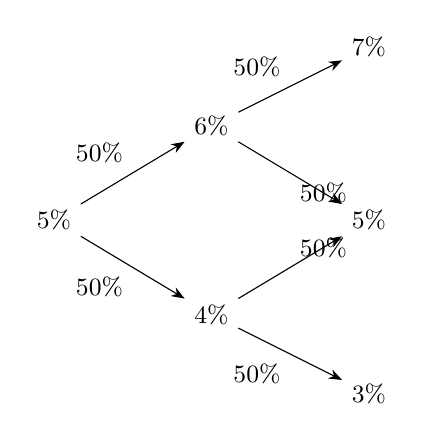
\begin{tikzpicture}[>=Stealth, node distance=2.5cm, every node/.style={font=\small}]
        % 节点
        \node (start) at (0,0) {5\%};
        \node (up1) at (2,1.2) {6\%};
        \node (down1) at (2,-1.2) {4\%};
        \node (uu) at (4,2.2) {7\%};
        \node (ud) at (4,0) {5\%};
        \node (dd) at (4,-2.2) {3\%};
    
        % 箭头
        \draw[->] (start) -- (up1) node[midway, above left] {50\%};
        \draw[->] (start) -- (down1) node[midway, below left] {50\%};
        \draw[->] (up1) -- (uu) node[midway, above left] {50\%};
        \draw[->] (up1) -- (ud) node[midway, below right] {50\%};
        \draw[->] (down1) -- (ud) node[midway, above right] {50\%};
        \draw[->] (down1) -- (dd) node[midway, below left] {50\%};
    \end{tikzpicture}

    If investors are risk-neutral, what is the price of a \$1 face value 2-year zero-coupon bond
today?
\end{question}

\begin{choices}
    \item \$0.90123.
    \item \$0.90567.
    \item \$0.90789.
    \item \$0.90832
\end{choices}

\begin{correctanswer}
    C
\end{correctanswer}

\begin{explanation}
 
    \textbf{C选项正确。}
    \begin{itemize}
        \item 根据风险中性定价模型：
        \begin{align*}
            p &= \left( \frac{1}{1.06} \times 0.5 + \frac{1}{1.04} \times 0.5 \right) \times 1.05 \\
            &= 0.90789
        \end{align*}
        \item 计算过程：
        \begin{itemize}
            \item 第一年：利率为6\%和4\%的概率各为50\%
            \item 第二年：利率为7\%、5\%、3\%的概率各为25\%、50\%、25\%
            \item 使用当前利率5\%进行折现
        \end{itemize}
    \end{itemize}
  
\end{explanation}
\checklist{
    掌握二叉树定价：考虑所有路径的概率和折现
}




\begin{question}
    A binomial interest-rate tree indicates a 1-year spot rate of 5\% and the price of the bond
    if rates decline is 96.50 and 94.25 if rates increase. The risk-neutral probability of an
    interest rate increase is 0.60. You hold a call option on the bond that expires in one year and
    has an exercise price of 94.00. The option value is closest to:
\end{question}

\begin{choices}
    \item 1.25.
    \item 1.05.
    \item 1.52.
    \item 1.45.
\end{choices}

\begin{correctanswer}
    D
\end{correctanswer}

\begin{explanation}
    \textbf{步骤1：确定参数}
    \begin{itemize}
        \item 看涨期权：执行价$K = 94.00$，1年到期
        \item 1年期即期利率：$r = 5\%$
        \item 风险中性概率：利率上升$p = 0.60$，利率下降$1-p = 0.40$
        \item 债券价格：利率上升时$P_u = 94.25$，利率下降时$P_d = 96.50$
    \end{itemize}

    \textbf{步骤2：计算各节点的期权收益}
    \begin{itemize}
        \item 利率上升时：$C_u = \max(P_u - K, 0) = \max(94.25 - 94.00, 0) = 0.25$
        \item 利率下降时：$C_d = \max(P_d - K, 0) = \max(96.50 - 94.00, 0) = 2.50$
    \end{itemize}

    \textbf{步骤3：计算风险中性下的期望收益并折现}
    \begin{itemize}
        \item 期权价值：
        \[
        C_0 = \frac{p \times C_u + (1-p) \times C_d}{1 + r} = \frac{0.60 \times 0.25 + 0.40 \times 2.50}{1.05} = \frac{1.15}{1.05} \approx 1.45
        \]
    \end{itemize}
\end{explanation}
\checklist{
    掌握期权定价：根据风险中性概率计算期望收益
}

\begin{question}
    Suppose an investor expects that the 1-year rate will remain at 5\% for the first year for a
    2-year zero-coupon bond. The investor also projects a 50\% probability that the 1-year spot rate
    will be 7\% in one year and a 50\% probability that the 1-year spot rate will be 3\% in one year.
    Which of the following inequalities most accurately reflects the convexity effect for this 2-
    year bond using Jensen's inequality formula?
\end{question}

\begin{choices}
    \item \$0.95238 > \$0.95200
    \item \$0.95200 > \$0.95000
    \item \$0.90703 > \$0.90667
    \item \$0.90703 > \$0.90690
\end{choices}

\begin{correctanswer}
    C
\end{correctanswer}

\begin{explanation}

\textbf{步骤1：理解凸性效应和Jensen不等式}
    \begin{itemize}
        \item 函数$f(r) = \frac{1}{1+r}$是凸函数（因为$f''(r) > 0$）。
        \item Jensen不等式：对于凸函数，$\mathbb{E}[f(X)] > f(\mathbb{E}[X])$。
        \item 因此：$\mathbb{E}\left[\frac{1}{1+r}\right] > \frac{1}{\mathbb{E}[1+r]}$。
    \end{itemize}

\textbf{步骤2：计算期望折现因子}
    \begin{itemize}
        \item 方法1（正确）：\[\mathbb{E}\left[\frac{1}{1+r}\right] = 0.5 \times \frac{1}{1.07} + 0.5 \times \frac{1}{1.03}
        = 0.5 \times 0.93458 + 0.5 \times 0.97087 = 0.95273
        \]
        \item 方法2（错误，忽略凸性）：\[\frac{1}{\mathbb{E}[1+r]} = \frac{1}{0.5 \times 1.07 + 0.5 \times 1.03} = \frac{1}{1.05} = 0.95238\]
    \end{itemize}

\textbf{步骤3：计算2年期债券价格}
    \begin{itemize}
        \item 使用正确方法：\[P_{\text{正确}} = \frac{0.95273}{1.05} = 0.90703\]
        \item 使用错误方法：\[P_{\text{错误}} = \frac{0.95238}{1.05} = 0.90667\]
    \end{itemize}

\textbf{结论}
    \begin{itemize}
        \item 凸性效应导致：$0.90703 > 0.90667$。
        \item 正确考虑利率不确定性时，债券价格更高，体现了凸性的价值。
    \end{itemize}
   
\end{explanation}
\checklist{
    理解凸性效应：Jensen不等式导致期望折现大于折现期望
}


\begin{question}
    Which of the following statements about puttable bonds compared to non-puttable bonds is
    false?
\end{question}

\begin{choices}
    \item They have less price volatility.
    \item They have positive convexity.
    \item Capital losses are capped as yields fall.
    \item At high yields, reinvestment rate risk rises.
\end{choices}

\begin{correctanswer}
    D
\end{correctanswer}

\begin{explanation}
    \textbf{A选项错误。}
    \begin{itemize}
        \item 可回售债券确实具有较小的价格波动性，因为回售权限制了价格下跌。
    \end{itemize}
    \textbf{B选项错误。}
    \begin{itemize}
        \item 可回售债券确实具有正凸性，因为回售权在利率上升时提供了额外的保护。
    \end{itemize}
    \textbf{C选项错误。}
    \begin{itemize}
        \item 可回售债券确实在收益率下降时限制了资本损失，因为投资者可以按回售价格卖出债券。
    \end{itemize}
    \textbf{D选项正确。}
    \begin{itemize}
        \item 可回售债券具有以下特征：
        \begin{itemize}
            \item 价格波动较小
            \item 正凸性
            \item 收益率下降时资本损失有限
            \item 收益率上升时再投资风险增加（而不是下降时）
        \end{itemize}
    \end{itemize}
\end{explanation}
\checklist{
    理解可回售债券：具有正凸性，限制下跌风险
}

\begin{question}
    Suppose a stock price is currently \$60.00 while the risk-free rate is 4.0\% per annum. For a
    series of options with a three month (0.25 years) maturity, the implied volatility is
    calculated at various strike prices, as below:
    \begin{itemize}
        \item Stock Price, S(0): \$60.00
        \item Risk-free rate: 4.0\%
        \item Maturity (years): 0.25
    \end{itemize}
\end{question}

\begin{choices}
    \item The market price (trades) of the put is \$4.20 and this is lower than the BSM model-based
    price which assumes an (ATM) volatility of 65.5\%
    \item The market price (trades) of the put is \$4.20 and this is higher than the BSM model-based
    price which assumes an (ATM) volatility of 65.5\%
    \item The market price (trades) of the put is \$5.25 and this is lower than the BSM model-based
    price which assumes an (ATM) volatility of 65.5\%
    \item The market price (trades) of the put is \$5.25 and this is equal to the BSM model-based price
    which assumes an (ATM) volatility of 65.5\%
\end{choices}

\begin{correctanswer}
    A
\end{correctanswer}

\begin{explanation}
    \textbf{A选项正确。}
    \begin{itemize}
        \item 根据看跌期权平价公式：
        \begin{align*}
            p &= c + Ke^{-rt} - S \\
            &= 8.75 + 55e^{-4\% \times 0.25} - 60 \\
            &= 4.20
        \end{align*}
        更高的波动率意味着更高的期权价格，因此市场价格低于BSM模型价格。
    \end{itemize}
\end{explanation}
\checklist{
    理解期权定价：波动率越高，期权价格越高
}


\begin{question}
    Which of the following factors is (are) reason(s) why the Black-Scholes-Merton option
    pricing model is not appropriate for valuing options on government bonds? \\
    I. Bonds have interest rate risk.\\ 
    II. Have an upper price bound.\\
    III. Bonds do not have constant price volatility. \\
    IV. Bonds are not priced by arbitrage.
\end{question}

\begin{choices}
    \item I and II.
    \item II and III.
    \item III and IV.
    \item IV only.
\end{choices}

\begin{correctanswer}
    B
\end{correctanswer}

\begin{explanation}
 \textbf{陈述I：不是主要原因。}
    \begin{itemize}
        \item 虽然债券有利率风险，但BSM模型可以处理标的资产的风险。
        \item BSM模型假设无风险利率为常数，但这不是其不适用于债券期权的主要原因。
    \end{itemize}

\textbf{陈述II：正确。}
    \begin{itemize}
        \item 债券价格存在上限：面值加上所有未付利息（到期时最多等于面值+利息总和）。
        \item BSM模型假设标的资产价格可以无限增长，这与债券价格有上限的特征不符。
    \end{itemize}

\textbf{陈述III：正确。}
    \begin{itemize}
        \item 债券价格波动率不是常数：随着到期时间临近，债券价格波动率会下降（因为价格收敛到面值）。
        \item BSM模型假设波动率为常数，这与债券波动率的时变特征不符。
    \end{itemize}

\textbf{陈述IV：错误。}
    \begin{itemize}
        \item 政府债券及其期权都可以通过无套利定价。
        \item 无套利定价是金融定价的基本原则，并非BSM模型不适用的原因。
    \end{itemize}
\end{explanation}
\checklist{
    理解BSM模型局限：债券价格有上限，波动率非常数
}


\begin{question}
    A European put option has two years to expiration and a strike price of \$101.00. The underlying asset is a three-year bond with a 7\% coupon rate. Assume that the risk-neutral probability of an up move is 0.76 in year 1 and 0.60 in year 2. The current interest rate is 3.00\%. At the end of year 1, the rate will either be 5.99\% or 4.44\%. If the rate in year 1 is 5.99\%, it will either rise to 8.56\% or rise to 6.34\% in year 2. If the rate in year 1 is 4.44\%, it will either rise to 6.34\% or rise to 4.70\%. The current value of the put option is closest to:
\end{question}

\begin{choices}
    \item \$1.17
    \item \$1.30
    \item \$1.49
    \item \$1.98
\end{choices}

\begin{correctanswer}
    A
\end{correctanswer}

\begin{explanation}
    \textbf{步骤1：计算第二年末各节点的期权价值}
    \begin{itemize}
        \item 第二年末债券还有1年到期，需支付本金和利息\$107
        \item 利率8.56\%：债券价格≈\$98.56，期权价值=\$2.44
        \item 利率6.34\%：债券价格≈\$100.62，期权价值=\$0.38
        \item 利率4.70\%：债券价格≈\$102.20，期权价值=\$0.00
    \end{itemize}

    \textbf{步骤2：计算第一年末各节点的期权价值}
    \begin{itemize}
        \item 上层节点（利率5.99\%）：
        \[
        V_{1u} = \frac{0.60 \times 2.44 + 0.40 \times 0.38}{1.0599} \approx \$1.52
        \]
        \item 下层节点（利率4.44\%）：
        \[
        V_{1d} = \frac{0.60 \times 0.38 + 0.40 \times 0.00}{1.0444} \approx \$0.22
        \]
    \end{itemize}

    \textbf{步骤3：计算当前期权价值}
    \begin{itemize}
        \item 当前期权价值：
        \[
        V_0 = \frac{0.76 \times 1.52 + 0.24 \times 0.22}{1.0300} \approx \$1.17
        \]
    \end{itemize}

\end{explanation}
\checklist{
    掌握二叉树模型：使用风险中性概率计算期权价值
}



\begin{question}
    An analyst at an investment bank is studying interest rate trees and how they are constructed and used to price fixed-income contingent claims under the no-arbitrage assumption. The analyst focuses on the characteristics and features of interest rate trees constructed using risk-neutral pricing. Which of the following is correct?
\end{question}

\begin{choices}
    \item Risk-neutral pricing assumes that the probabilities of both up and down states equal 0.5, reflecting a neutral view on the direction of interest rate movements.
    \item Risk-neutral pricing requires creating a new interest rate tree for each fixed-income contingent claim.
    \item Risk-neutral pricing makes the expected discounted value of fixed-income contingent claims equal to their market prices.
    \item Risk-neutral pricing requires constructing and pricing a replicating portfolio for contingent claims, even when the risk-neutral tree for interest rates is known.
\end{choices}

\begin{correctanswer}
    C
\end{correctanswer}

\begin{explanation}
    \textbf{A选项错误。}
    \begin{itemize}
        \item 风险中性概率不一定等于0.5，它们是通过使标的证券价格等于其预期折现价值来确定的。
    \end{itemize}
    \textbf{B选项错误。}
    \begin{itemize}
        \item 风险中性定价是一种非常高效的方法，可以在相同的假设利率过程下对多个或有权益进行定价。
    \end{itemize}
    \textbf{C选项正确。}
    \begin{itemize}
        \item 风险中性定价的核心是找到使标的证券价格等于其预期折现价值的风险中性概率。
    \end{itemize}
    \textbf{D选项错误。}
    \begin{itemize}
        \item 一旦已知利率的风险中性树，就可以直接对任何或有权益进行定价，无需构建和定价其复制组合。
    \end{itemize}
\end{explanation}
\checklist{
    理解风险中性定价：使预期折现价值等于市场价格
}




\section{考点2:预期、风险溢价、凸性和期限结构的形状}
\setcounter{question}{0}

\begin{question}
    If all other factors remain unchanged, what happens to the price-yield curve of a zero-coupon bond as its maturity increases?
\end{question}

\begin{choices}
    \item The curve becomes flatter.
    \item The curve becomes steeper.
    \item The curve becomes less convex.
    \item The curve becomes more convex.
\end{choices}

\begin{correctanswer}
    D
\end{correctanswer}

\begin{explanation}
    \textbf{A选项错误。} 
    \begin{itemize}
        \item 随着期限增加，价格-收益率曲线不会变得更平坦，而是凸性增强。
    \end{itemize}
    \textbf{B选项错误。} 
    \begin{itemize}
        \item 曲线变陡并不是主要特征，主要是凸性变化。
    \end{itemize}
    \textbf{C选项错误。} 
    \begin{itemize}
        \item 期限越长，凸性越大，不会变得更不凸。
    \end{itemize}
    \textbf{D选项正确。} 
    \begin{itemize}
        \item 随着零息债券期限的增加，价格-收益率曲线的凸性增强。
    \end{itemize}
\end{explanation}
\checklist{凸性与期限}



\begin{question}
    Suppose an investor anticipates that the 1-year zero-coupon bond rate will stay at 6\% this year, rise to 8\% next year, and reach 10\% in the third year. What is the 3-year spot rate for a zero-coupon bond with a face value of \$1, assuming all investors share the same expectations for future 1-year rates?
\end{question}

\begin{choices}
    \item 7.888\%
    \item 7.988\%
    \item 8.000\%
    \item 8.088\%
\end{choices}

\begin{correctanswer}
    B
\end{correctanswer}

\begin{explanation}
    
    \textbf{步骤1：理解即期利率的计算}
    \begin{itemize}
        \item 3年期即期利率是将1年期远期利率序列按复利几何平均得到。
        \item 根据期望理论，3年期零息债券的现值应等于按1年期远期利率序列折现的现值。
    \end{itemize}

    \textbf{步骤2：建立等价关系}
    \begin{itemize}
        \item 按3年期即期利率折现：\[\frac{\$1}{(1 + r_3)^3}\]
        \item 按1年期远期利率序列折现：\[\frac{\$1}{1.06 \times 1.08 \times 1.10}\]
        \item 两者相等：\[\frac{\$1}{(1 + r_3)^3} = \frac{\$1}{1.06 \times 1.08 \times 1.10}\]
    \end{itemize}

    \textbf{步骤3：计算3年期即期利率}
    \begin{itemize}
        \item 整理方程：
        \[
        (1 + r_3)^3 = 1.06 \times 1.08 \times 1.10 = 1.25928
        \]
        \item 求解：
        \[
        r_3 = \sqrt[3]{1.25928} - 1 = 1.07988 - 1 = 0.07988 = 7.988\%
        \]
    \end{itemize}
    
   
\end{explanation}
\checklist{即期利率计算}






\begin{question}
    If all other factors remain constant, what happens to the bond price-yield curve as the maturity of a zero-coupon bond increases? The pricing curve becomes:
\end{question}

\begin{choices}
    \item less concave.
    \item more concave.
    \item less convex.
    \item more convex.
\end{choices}

\begin{correctanswer}
    D
\end{correctanswer}

\begin{explanation}
    \textbf{A选项错误。} 
    \begin{itemize}
        \item 随着期限增加，曲线不会变得更凹。
    \end{itemize}
    
    \textbf{B选项错误。} 
    \begin{itemize}
        \item 曲线的主要变化是凸性增强，而非凹性。
    \end{itemize}
    
    \textbf{C选项错误。} 
    \begin{itemize}
        \item 期限越长，凸性越大，不会变得更不凸。
    \end{itemize}
    
    \textbf{D选项正确。} 
    \begin{itemize}
        \item 随着零息债券期限增加，价格-收益率曲线凸性增强。
    \end{itemize}
\end{explanation}
\checklist{凸性与期限关系}


\begin{question}
    A market risk manager seeks to calculate the price of a two-year zero-coupon bond. The one-year interest rate today is 10.0\%. There is a 50\% probability that the interest rate will be
    12.0\% and a 50\% probability that it will be 8.0\% in one year. Assuming that the risk premium of
    duration risk is 50 basis points each year, and that the face value is EUR 1000, which of the
    following should be the price of the zero-coupon bond?
    
\end{question}

\begin{choices}
    \item EUR 822.98
    \item EUR 826.44
    \item EUR 826.72
    \item EUR 921.66
\end{choices}

\begin{correctanswer}
    B
\end{correctanswer}

\begin{explanation}
    \textbf{步骤1：确定参数}
    \begin{itemize}
        \item 2年期零息债券，面值EUR 1{,}000
        \item 当前1年期利率：$r_0 = 10.0\%$
        \item 1年后利率：50\%概率为12.0\%，50\%概率为8.0\%
        \item 期限风险溢价：每年50个基点（0.5\%）
    \end{itemize}

    \textbf{步骤2：计算调整后的折现率}
    \begin{itemize}
        \item 第1年折现率：$10.0\% + 0.5\% = 10.5\%$（考虑风险溢价）
        \item 如果第2年利率为12.0\%：折现率$= 12.0\% + 0.5\% = 12.5\%$
        \item 如果第2年利率为8.0\%：折现率$= 8.0\% + 0.5\% = 8.5\%$
    \end{itemize}

    \textbf{步骤3：计算债券价格}
    \begin{itemize}
        \item 使用风险中性定价，计算期望折现值：
        \[
        \begin{aligned}
        P &= \frac{1}{1.105} \times \left[0.5 \times \frac{1}{1.125} + 0.5 \times \frac{1}{1.085}\right] \times 1{,}000 \\
        &= \frac{1}{1.105} \times \left[0.5 \times 0.8889 + 0.5 \times 0.9217\right] \times 1{,}000 \\
        &= \frac{1}{1.105} \times 0.9053 \times 1{,}000 \\
        &= 0.8264 \times 1{,}000 \\
        &= \text{EUR }826.44
        \end{aligned}
        \]
    \end{itemize}
  
   
\end{explanation}
\checklist{零息债定价与风险溢价}

\begin{question}
    A fixed-income analyst is asked to determine the price of a 3-year zero-coupon bond, given the following market conditions: current interest rate is 2\%, annual interest rate volatility is 40 bps, and investors require an annual risk premium of 10 bps. What is the current price of the 3-year zero-coupon bond under these conditions?
\end{question}

\begin{choices}
    \item 0.9396
    \item 0.9410
    \item 0.9415
    \item 0.9424
\end{choices}

\begin{correctanswer}
    A
\end{correctanswer}

\begin{explanation}
    \textbf{步骤1：确定参数}
    \begin{itemize}
        \item 3年期零息债券，面值假设为\$1
        \item 当前利率：$r = 2\% = 0.02$
        \item 年利率波动率：$\sigma = 40 \text{ bps} = 0.40\% = 0.004$
        \item 年风险溢价：$\lambda = 10 \text{ bps} = 0.10\% = 0.001$
    \end{itemize}

    \textbf{步骤2：计算调整后的折现率}
    \begin{itemize}
        \item 考虑风险溢价后，折现率需要调整：$r_{\text{adj}} = r + \lambda = 0.02 + 0.001 = 0.021$
        \item 基础折现值：$P_{\text{base}} = \frac{1}{(1.021)^3} \approx 0.9415$
    \end{itemize}

    \textbf{步骤3：考虑凸性效应和波动率影响}
    \begin{itemize}
        \item 综合调整后的折现率需要考虑波动率的平方项（方差项）：
        \[
        r_{\text{total}} = r + \lambda + \frac{\sigma^2 \times T}{2}
        \]
        \item 对于3年期债券：$r_{\text{total}} = 0.02 + 0.001 + \frac{0.004^2 \times 3}{2} = 0.021 + 0.000024 = 0.021024$
        \item 债券价格：
        \[
        P = \frac{1}{(1 + r_{\text{total}})^3} = \frac{1}{(1.021024)^3} \approx 0.9396
        \]
    \end{itemize}
    
\end{explanation}
\checklist{零息债定价与风险溢价}

疑惑：这个波动率怎么用上的，这个的公式是什么。感觉不用上波动率也可以得出A。


\section{考点3:期限结构模型：漂移和波动性分布}
\setcounter{question}{0}

\begin{question}
    Tuckman's Model 1 assumes zero drift and is also called the normal model. Model 2 adds a drift term. According to Tuckman, each of the following statements about these two models is correct EXCEPT:
\end{question}

\begin{choices}
    \item A weakness of Model 1 (normal model) is that the short-term rate can become negative.
    \item Model 1 implies a term structure that is perfectly flat at the current rate for all maturities, including the long-term rates.
    \item Model 2 is more capable of producing an upward-sloping term structure, which is often observed.
    \item Model 2 is an equilibrium model, rather than an arbitrage-free model, because no attempt is made to match the term structure closely.
\end{choices}

\begin{correctanswer}
    B
\end{correctanswer}

\begin{explanation}
    \textbf{A选项错误。} 
    \begin{itemize}
        \item Model 1允许短期利率变为负值，确实是其缺陷之一。
    \end{itemize}
    
    \textbf{B选项正确。} 
    \begin{itemize}
        \item Model 1只在短期内表现为平坦结构，整体上由于凸性效应会导致期限结构向下倾斜。
    \end{itemize}
    
    \textbf{C选项错误。} 
    \begin{itemize}
        \item Model 2引入漂移项，更能生成现实中常见的上升期限结构。
    \end{itemize}
    
    \textbf{D选项错误。} 
    \begin{itemize}
        \item Model 2为均衡模型，确实未严格拟合实际期限结构。
    \end{itemize}
\end{explanation}
\checklist{模型1与模型2比较}


\begin{question}
    The Bureau of Labor Statistics has just reported an unexpected short-term increase in high-priced luxury automobiles. What is the most likely anticipated impact on a mean-reverting model of interest rates?
\end{question}

\begin{choices}
    \item The economic information is long-lived with a low mean reversion parameter.
    \item The economic information is short-lived with a low mean reversion parameter.
    \item The economic information is long-lived with a high mean reversion parameter.
    \item The economic information is short-lived with a high mean reversion parameter.
\end{choices}

\begin{correctanswer}
    D
\end{correctanswer}

\begin{explanation}
    \textbf{A选项错误。} 
    \begin{itemize}
        \item 该经济信息属于短期影响，不是长期。
    \end{itemize}
    
    \textbf{B选项错误。} 
    \begin{itemize}
        \item 虽然是短期信息，但均值回复参数应高而非低。
    \end{itemize}
    \textbf{C选项错误。} 
    \begin{itemize}
        \item 信息不是长期影响，均值回复参数高不适用。
    \end{itemize}
    \textbf{D选项正确。} 
    \begin{itemize}
        \item 该经济消息时效短，均值回复参数高，调整速度快。
    \end{itemize}
\end{explanation}
\checklist{均值回复与经济消息}


\begin{question}
    An analyst is building a short-term interest rate tree according to the Vasicek Model which
    is characterized by mean reversion. t = 1/12. The current short-term rate is 8.00\%. The annual
    volatility is 200bps. The central tendency is 3.00\%. The speed of mean reversion is equal to 0.60. Here is his rate tree:

\begin{center}
    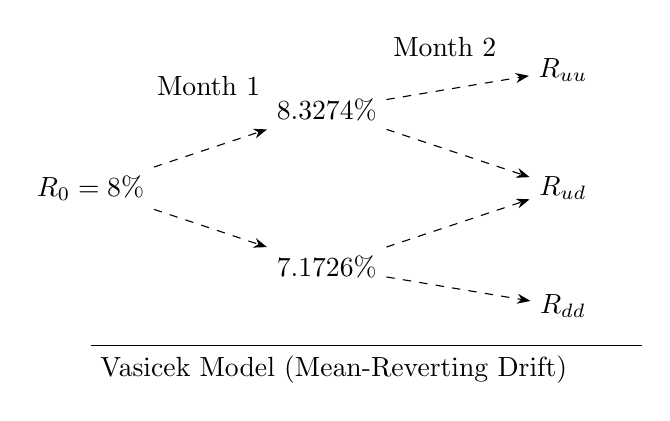
\begin{tikzpicture}[>=Stealth, node distance=2.5cm]
        % 节点
        \node (start) at (0,0) {$R_0 = 8\%$};
        \node (up1)   at (3,1) {8.3274\%};
        \node (down1) at (3,-1) {7.1726\%};
        \node (uu) at (6,1.5) {$R_{uu}$};
        \node (ud) at (6,0)   {$R_{ud}$};
        \node (dd) at (6,-1.5) {$R_{dd}$};
    
        % 箭头
        \draw[->, dashed] (start) -- (up1);
        \draw[->, dashed] (start) -- (down1);
        \draw[->, dashed] (up1) -- (uu);
        \draw[->, dashed] (up1) -- (ud);
        \draw[->, dashed] (down1) -- (ud);
        \draw[->, dashed] (down1) -- (dd);
    
        % 标签
        \node at (1.5,1.3) {Month 1};
        \node at (4.5,1.8) {Month 2};
        \draw (0,-2) -- (7,-2); % 上方横线
        \node[anchor=west] at (0,-2.3) {Vasicek Model (Mean-Reverting Drift)};
    \end{tikzpicture}
\end{center}

    What is the value in the Vasicek tree for Rud?
\end{question}

\begin{choices}
    \item 6.833\%
    \item 7.513\%
    \item 8.019\%
    \item 9.225\%
\end{choices}

\begin{correctanswer}
    B
\end{correctanswer}

\begin{explanation}

    \textbf{B选项正确。}
    \begin{itemize}
        \item In month 2:
        \[
r_{ud} = r_u + k(\theta - r_u)dt - \sigma \sqrt{dt}
= 8.3274\% + 0.6 \times \frac{3\% - 8.3274\%}{12} - 0.02 \times \sqrt{\frac{1}{12}}
= 7.484\%
\]

\[
r_{du} = r_d + k(\theta - r_d)dt + \sigma \sqrt{dt}
= 7.1726\% + 0.6 \times \frac{3\% - 7.1726\%}{12} + 0.02 \times \sqrt{\frac{1}{12}}
= 7.541\%
\]

\[
\Rightarrow \frac{7.484\% + 7.541\%}{2} = 7.513\%
\]
    \end{itemize}
   
\end{explanation}
\checklist{Vasicek模型利率树计算}


\begin{question}
    Using Model 2, suppose the current short-term rate is 8\%, the annual drift is 50bps, and the short-term rate standard deviation is 2\%. If the ex-post realization of the dw random variable is 0.3, after constructing a 2-period interest rate tree with annual periods, what is the interest rate at the middle node at the end of year 2?
\end{question}

\begin{choices}
    \item 8.0\%
    \item 8.8\%
    \item 9.0\%
    \item 9.6\%
\end{choices}

\begin{correctanswer}
    C
\end{correctanswer}

\begin{explanation}
    \textbf{步骤1：理解Model 2的利率树结构}
    \begin{itemize}
        \item Model 2公式：$dr = \lambda dt + \sigma dw$
        \item 其中：$\lambda = 0.5\%$（年漂移），$\sigma = 2\%$（标准差），$dt = 1$年
    \end{itemize}

    \textbf{步骤2：理解中间节点的特性}
    \begin{itemize}
        \item 在2期利率树中，第2年末的中间节点是两条路径的汇合点。
        \item 一条路径：先上升后下降（$+dw - dw$）
        \item 另一条路径：先下降后上升（$-dw + dw$）
        \item 在中间节点，随机项$dw$互相抵消，只剩下漂移项的累积效应。
    \end{itemize}

    \textbf{步骤3：计算中间节点的利率}
    \begin{itemize}
        \item 中间节点利率公式：
        \[
        r_{\text{mid}} = r_0 + 2 \times \lambda \times dt
        \]
        \item 代入数值：
        \[
        r_{\text{mid}} = 8\% + 2 \times 0.5\% \times 1 = 8\% + 1\% = 9.0\%
        \]
        \item 由于$dw$项在中间节点抵消，$dw = 0.3$的实现在中间节点不产生影响。
    \end{itemize}
\end{explanation}
\checklist{Model 2利率树计算}


\begin{question}
    An analyst is constructing an interest rate tree with monthly time steps (t = 1/12). The current short-term rate is 4.0\%. The term structure model assumes an annual basis point volatility of 180bps. Using Model 1 (normally distributed rates, zero drift), what is the interest rate at the uppermost node at the end of month 2?
\end{question}

\begin{choices}
    \item 4.20\%
    \item 4.83\%
    \item 5.04\%
    \item 6.59\%
\end{choices}

\begin{correctanswer}
    C
\end{correctanswer}

\begin{explanation}
    \textbf{C选项正确：} 
    \begin{itemize}
        \item 按Model 1，第二个月最上节点利率为：
        \[
        r = r_0 + 2\sigma\sqrt{dt} = 4\% + 2 \times 0.018 \times \sqrt{\frac{1}{12}} \approx 5.04\%
        \]
        \item 其中，\(\sigma = 180\)bps = 0.018，\(dt = 1/12\)。两期上升路径需叠加两次标准差项，得出5.04\%。
    \end{itemize}
\end{explanation}
\checklist{Model 1利率树计算}


\begin{question}
    An analyst constructed an interest rate tree with monthly time steps (t = 1/12). The current short-term rate is 3.0\%. The term structure model assumes an annual basis point volatility of 200bps and an annual drift of 50bps. Using Model 2 (normally distributed rates with drift), what is the missing value at the lowest node at the end of month 2?
\end{question}

\begin{choices}
    \item 1.93\%
    \item 2.17\%
    \item 2.38\%
    \item 3.01\%
\end{choices}

\begin{correctanswer}
    A
\end{correctanswer}

\begin{explanation}
    \textbf{A选项正确。}
    \begin{itemize}  
    \item 计算最低节点利率时，需两次向下移动，每次都要减去波动项并加上漂移项。  
    \item 计算公式为：  
    \[
    r = r_0 + 2 \times \lambda \times dt - 2 \times \sigma \sqrt{dt}
    \]
    \item 其中，\( r_0 = 3.0\% \)，\( \lambda = 0.5\% = 0.005 \)，\( \sigma = 2.0\% = 0.02 \)，\( dt = 1/12 \)。  
    \[
    r = 3.0\% + 2 \times 0.005 \times \frac{1}{12} - 2 \times 0.02 \times \sqrt{\frac{1}{12}}
    \]
    \[
    = 3.0\% + 0.000833 - 0.011547 \approx 1.93\%
    \]
   \end{itemize}

\end{explanation}
\checklist{Model 2利率树节点计算}



\begin{question}
    The current short-term rate is 4.00\%. Under a Ho-Lee Model with time-dependent drift, the
    time step is monthly and the annualized drifts are as follows: +100bps in the first month and
    +80bps in the second month. The annual basis point volatility is 200bps.
\begin{center}
    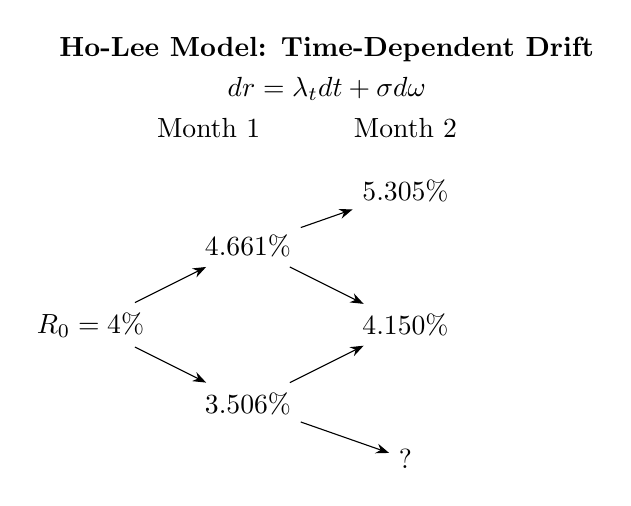
\begin{tikzpicture}[>=Stealth, node distance=2.5cm]
        % 标题
        \node at (3,5) {\textbf{Ho-Lee Model: Time-Dependent Drift}};
        \node at (3,4.5) {$dr = \lambda_t dt + \sigma d\omega$};
    
        % 节点
        \node (start) at (0,1.5) {$R_0 = 4\%$};
        \node (up1)   at (2,2.5) {4.661\%};
        \node (down1) at (2,0.5) {3.506\%};
        \node (uu) at (4,3.2) {5.305\%};
        \node (ud) at (4,1.5) {4.150\%};
        \node (dd) at (4,-0.2) {?};
    
        % 箭头
        \draw[->] (start) -- (up1);
        \draw[->] (start) -- (down1);
        \draw[->] (up1) -- (uu);
        \draw[->] (up1) -- (ud);
        \draw[->] (down1) -- (ud);
        \draw[->] (down1) -- (dd);
    
        % 月份标签
        \node at (1.5,4) {Month 1};
        \node at (4,4) {Month 2};
    \end{tikzpicture}
\end{center}
    What is the value of the missing node?

\end{question}

\begin{choices}
    \item 2.447\%
    \item 2.677\%
    \item 2.995\%
    \item 3.256\%
\end{choices}

\begin{correctanswer}
    C
\end{correctanswer}

\begin{explanation}

   \textbf{步骤1：确定参数}
        \begin{itemize}
            \item 当前利率：$r_0 = 4.0\%$
            \item 第1个月漂移：$\lambda_1 = 100 \text{ bps} = 0.01$
            \item 第2个月漂移：$\lambda_2 = 80 \text{ bps} = 0.008$
            \item 年波动率：$\sigma = 200 \text{ bps} = 0.02$
            \item 时间步长：$dt = \frac{1}{12}$
        \end{itemize}

   \textbf{步骤2：计算dd节点（两期都下降）的利率}
        \begin{itemize}
            \item Ho-Lee模型：$dr = \lambda_t dt + \sigma d\omega$
            \item dd节点意味着两期都下降（$-dw, -dw$），所以：
            \[
            r_{dd} = r_0 + (\lambda_1 + \lambda_2)dt - 2\sigma\sqrt{dt}
            \]
            \item 代入数值：
            \[
            r_{dd} = 4\% + \frac{0.01 + 0.008}{12} - 2 \times 0.02 \times \sqrt{\frac{1}{12}} = 4\% + 0.0015 - 0.01155 = 2.995\%
            \]
        \end{itemize}


\end{explanation}
\checklist{Ho-Lee模型利率树计算}


\begin{question}
    A risk manager is pricing a 10-year call option on 10-year Treasuries using a successfully tested pricing model. Current interest rate volatility is high and the risk manager is concerned about the effect this may have on short-term rates when pricing the option. Which of the following actions would best address the potential for negative short-term interest rates to arise in the model?
\end{question}

\begin{choices}
    \item The risk manager uses a normal distribution of interest rates.
    \item When short-term rates are negative, the risk manager adjusts the risk-neutral probabilities.
    \item When short-term rates are negative, the risk manager increases the volatility.
    \item When short-term rates are negative, the risk manager sets the rate to zero.
\end{choices}

\begin{correctanswer}
    D
\end{correctanswer}

\begin{explanation}
    \textbf{A选项错误。}
    \begin{itemize}
        \item 采用正态分布本身无法避免负利率的出现，反而可能导致负利率节点增多。
    \end{itemize}

    \textbf{B选项错误。} 
    \begin{itemize}
        \item 调整风险中性概率会影响整个利率树的动态，不仅仅局限于负利率节点，反而可能带来更多模型偏差。
    \end{itemize}

    \textbf{C选项错误。} 
    \begin{itemize}
        \item 增加波动率会使利率分布更分散，反而可能增加负利率出现的概率，不能解决根本问题。
    \end{itemize}

    \textbf{D选项正确。} 
    \begin{itemize}
        \item 当模型中出现负短期利率时，将其设为零是常用且有效的处理方法。这样可以局部修正负利率节点，同时保留其他节点的原始结构，经济含义也更合理。负利率虽然在某些模型下可能出现，但实际市场中投资者一般不会以负利率出借资金，因此将负利率设为零更符合实际情况。
    \end{itemize}
\end{explanation}
\checklist{负利率处理方法}


\begin{question}
    Regarding the validity of time-dependent drift models, which of the following statements is(are) correct? 

    I. Time-dependent drift models are flexible since volatility from period to period can change. However, volatility must be an increasing function of short-term rate volatilities. 

    II. Time-dependent volatility functions are useful for pricing interest rate caps and floors.
\end{question}

\begin{choices}
    \item I only.
    \item II only.
    \item Both I and II.
    \item Neither I nor II.
\end{choices}

\begin{correctanswer}
    B
\end{correctanswer}

\begin{explanation}
    \textbf{陈述I：错误。}
        \begin{itemize}
            \item 时间相关漂移模型允许波动率在不同时期变化，具有灵活性。但波动率不必须是短期利率波动率的递增函数。
            \item 波动率可以是递增、递减或恒定的，取决于模型设定和市场条件。因此，陈述I的后半部分（"必须递增"）是错误的。
        \end{itemize}

        \textbf{陈述II：正确。}
        \begin{itemize}
            \item 时间相关波动率函数对利率上限和下限的定价很有用。
            \item 原因：
            \begin{itemize}
                \item 利率上限和下限涉及多期支付（每期都可能触发）
                \item 不同时期的波动率可能不同（如短期波动率较高，长期波动率较低）
                \item 时间相关的波动率设定能更准确地捕捉不同时期的波动特征
            \end{itemize}
        \end{itemize}
\end{explanation}
\checklist{时间相关波动率模型}


\begin{question}
    Which of the following statements best characterizes the differences between the Ho-Lee model with drift and the lognormal model with drift?
\end{question}

\begin{choices}
    \item In the Ho-Lee model and the lognormal model the drift terms are multiplicative.
    \item In the Ho-Lee model and the lognormal model the drift terms are additive.
    \item In the Ho-Lee model the drift terms are multiplicative, but in the lognormal model the drift terms are additive.
    \item In the Ho-Lee model the drift terms are additive, but in the lognormal model the drift terms are multiplicative.
\end{choices}

\begin{correctanswer}
    D
\end{correctanswer}

\begin{explanation}
    \textbf{A选项错误。} 
    \begin{itemize}
    \item 两个模型的漂移项累积方式并非都是相乘。
    \end{itemize}
    \textbf{B选项错误。} 
    \begin{itemize}
    \item 两个模型的漂移项累积方式并非都是相加。
    \end{itemize}

    \textbf{C选项错误。} 
    \begin{itemize}
    \item Ho-Lee模型是相加，lognormal模型是相乘，顺序颠倒。
    \end{itemize}

    \textbf{D选项正确。} 
    \begin{itemize}
    \item Ho-Lee模型的漂移项累积是相加的，lognormal模型的漂移项累积是相乘的。Ho-Lee模型允许每期漂移项变化，累积效果为加法；而对数正态模型累积效果为乘法。
    \end{itemize}
\end{explanation}
\checklist{Ho-Lee模型与对数正态模型}



\begin{question}
    Lisa Wang, CFA, is discussing the appropriate usage of mean-reverting models relative to no-drift models, models that incorporate drift, and Black-Kim models. Wang makes the following statements: 
    \begin{itemize}
        \item Statement 1: Both Model 1 (no drift) and the CIR model assume parallel shifts from changes in the short-term rate. 
        \item Statement 2: The CIR model assumes decreasing volatility of future short-term rates while Model 1 assumes constant volatility of future short-term rates. 
        \item Statement 3: The constant drift model (Model 2) is a more flexible model than the Black-Kim model. 
    \end{itemize}
    How many of her statements are correct?
\end{question}

\begin{choices}
    \item 0
    \item 1
    \item 2
    \item 3
\end{choices}

\begin{correctanswer}
    B
\end{correctanswer}

\begin{explanation}
    \textbf{A选项错误：} 实际上有一条陈述是正确的。

    \textbf{B选项正确：} 只有Statement 2是正确的。CIR模型假设未来短期利率的波动性递减，而Model 1假设波动性恒定。Statement 1错误，因为CIR模型不一定是平行移动；Statement 3错误，因为Black-Kim模型比Model 2更通用，Model 2只是Black-Kim模型的特例。

    \textbf{C选项错误：} 只有一条陈述正确，不是两条。

    \textbf{D选项错误：} 只有一条陈述正确，不是三条。
\end{explanation}
\checklist{利率模型特性比较}


\begin{question}
    Using Model 1, suppose the current short-term interest rate is 5\%, annual volatility is 80bps, and dw, a normally distributed random variable with mean 0 and standard deviation \(\sqrt{dt}\), has an expected value of zero. After one month, the realization of dw is -0.5. What is the change in the spot rate and the new spot rate?
\end{question}

\begin{choices}
    \item 0.4\%, 5.4\%
    \item -0.4\%, 4.6\%
    \item 0.8\%, 5.8\%
    \item -0.8\%, 4.2\%
\end{choices}

\begin{correctanswer}
    B
\end{correctanswer}

\begin{explanation}
    \textbf{A选项错误：} 该选项将变化方向搞反，dw为负时应为利率下降。

    \textbf{B选项正确：} Model 1为无漂移模型，利率变化公式为 \( dr = \sigma dw \)。已知年化波动率为0.8\%，一个月的dw为-0.5，则
    \[
    dr = 0.8\% \times (-0.5) = -0.4\%
    \]
    初始利率为5\%，新即期利率为
    \[
    5\% + (-0.4\%) = 4.6\%
    \]
    计算过程和结果均正确。

    \textbf{C选项错误：} 该选项将dw的符号和倍数搞错，结果偏高。

    \textbf{D选项错误：} 该选项将dw的绝对值扩大，未按题意计算。
\end{explanation}
\checklist{无漂移模型利率变动}

\begin{question}
    An analyst is constructing an interest rate tree with monthly time steps; i.e., \( t = 1/12 \). The current short-term rate is 3.5\%. His term structure model assumes an annual basis point volatility of 150bps. He employs Model 1 which assumes normally distributed rates and zero drift. Here is his rate tree:


    \begin{figure}[H]
        \centering
        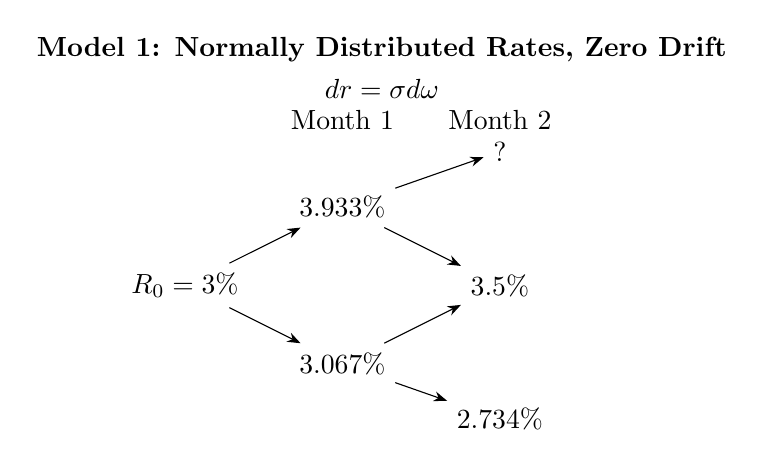
\begin{tikzpicture}[>=Stealth, node distance=2.5cm]
            % 标题
            \node at (2.5,4.5) {\textbf{Model 1: Normally Distributed Rates, Zero Drift}};
            \node at (2.5,4) {$dr = \sigma d\omega$};
    
            % 节点
            \node (start) at (0,1.5) {$R_0 = 3\%$};
            \node (up1)   at (2,2.5) {3.933\%};
            \node (down1) at (2,0.5) {3.067\%};
            \node (uu) at (4,3.2) {?};
            \node (ud) at (4,1.5) {3.5\%};
            \node (dd) at (4,-0.2) {2.734\%};
    
            % 箭头
            \draw[->] (start) -- (up1);
            \draw[->] (start) -- (down1);
            \draw[->] (up1) -- (uu);
            \draw[->] (up1) -- (ud);
            \draw[->] (down1) -- (ud);
            \draw[->] (down1) -- (dd);
    
            % 月份标签
            \node at (2,3.6) {Month 1};
            \node at (4,3.6) {Month 2};
        \end{tikzpicture}
    \end{figure}


    What is the un-displayed missing value?
\end{question}

\begin{choices}
    \item 3.933\%
    \item 4.366\%
    \item 4.150\%
    \item 4.600\%
\end{choices}

\begin{correctanswer}
    B
\end{correctanswer}

\begin{explanation}
   

    \textbf{步骤1：确定参数}
    \begin{itemize}
        \item 当前短期利率：$r_0 = 3.5\%$（题目中给出）
        \item 年波动率：$\sigma = 150 \text{ bps} = 1.5\% = 0.015$
        \item 时间步长：$dt = \frac{1}{12}$（月）
        \item Model 1：零漂移（$\lambda = 0$），只有随机项
    \end{itemize}

    \textbf{步骤2：理解uu节点（最上节点）的特性}
    \begin{itemize}
        \item uu节点意味着两期都上升（$+dw, +dw$）。
        \item 每期上升幅度：$\sigma \sqrt{dt} = 0.015 \times \sqrt{\frac{1}{12}} \approx 0.015 \times 0.2887 \approx 0.00433 = 0.433\%$
    \end{itemize}

    \textbf{步骤3：计算uu节点的利率}
    \begin{itemize}
        \item 最上节点利率：
        \[
        r_{uu} = r_0 + 2 \times \sigma \sqrt{dt} = 3.5\% + 2 \times 0.00433 = 3.5\% + 0.866\% = 4.366\%
        \]
    \end{itemize}
   
\end{explanation}
\checklist{Model 1利率树节点计算}







\begin{question}
    An analyst constructed an interest rate tree with monthly time steps, where t = 1/12. The
    current short-term rate is 3.0\%. His term structure model assumes an annual basis point
    volatility of 200bps with an annual drift of 50bps. He employs Model 2 which assumes normally
    distributed rates and incorporating drift. Here is his rate tree:

    \begin{figure}[H]
        \centering
        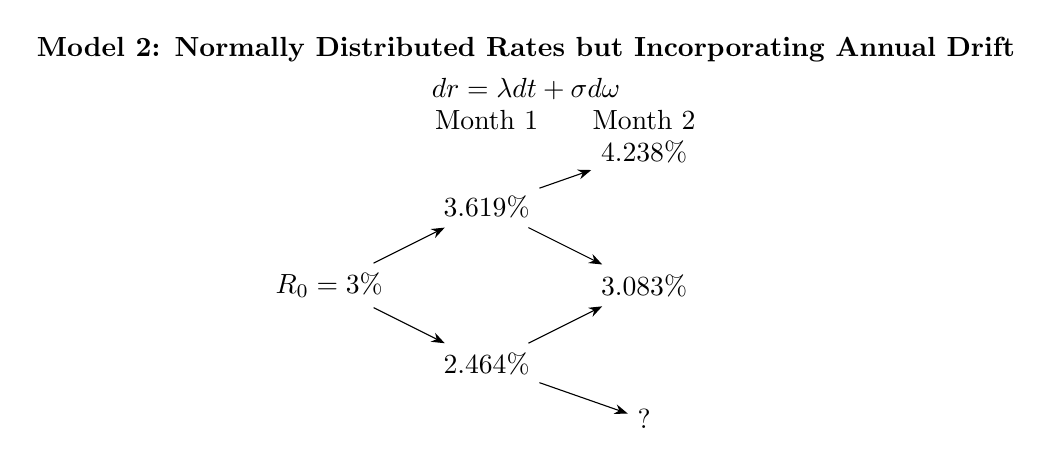
\begin{tikzpicture}[>=Stealth, node distance=2.5cm]
            % 标题
            \node at (2.5,4.5) {\textbf{Model 2: Normally Distributed Rates but Incorporating Annual Drift}};
            \node at (2.5,4) {$dr = \lambda dt + \sigma d\omega$};
    
            % 节点
            \node (start) at (0,1.5) {$R_0 = 3\%$};
            \node (up1)   at (2,2.5) {3.619\%};
            \node (down1) at (2,0.5) {2.464\%};
            \node (uu) at (4,3.2) {4.238\%};
            \node (ud) at (4,1.5) {3.083\%};
            \node (dd) at (4,-0.2) {?};
    
            % 箭头
            \draw[->] (start) -- (up1);
            \draw[->] (start) -- (down1);
            \draw[->] (up1) -- (uu);
            \draw[->] (up1) -- (ud);
            \draw[->] (down1) -- (ud);
            \draw[->] (down1) -- (dd);
    
            % 月份标签
            \node at (2,3.6) {Month 1};
            \node at (4,3.6) {Month 2};
        \end{tikzpicture}
    \end{figure}

    What is the un-displayed missing value?
\end{question}

\begin{choices}
    \item 1.93\%
    \item 2.17\%
    \item 2.38\%
    \item 3.01\%
\end{choices}

\begin{correctanswer}
    A
\end{correctanswer}

\begin{explanation}
 \textbf{步骤1：确定参数}
    \begin{itemize}
        \item 当前短期利率：$r_0 = 3.0\%$
        \item 年漂移：$\lambda = 50 \text{ bps} = 0.5\% = 0.005$
        \item 年波动率：$\sigma = 200 \text{ bps} = 2.0\% = 0.02$
        \item 时间步长：$dt = \frac{1}{12}$（月）
        \item Model 2：$dr = \lambda dt + \sigma d\omega$
    \end{itemize}

    \textbf{步骤2：理解dd节点（最下节点）的特性}
    \begin{itemize}
        \item dd节点意味着两期都下降（$-dw, -dw$）。
        \item 需要加上两期的漂移项，减去两期的随机项。
    \end{itemize}

    \textbf{步骤3：计算dd节点的利率}
    \begin{itemize}
        \item 最下节点利率公式：
        \[
        r_{dd} = r_0 + 2\lambda dt - 2\sigma\sqrt{dt}
        \]
        \item 代入数值：
        \[
        r_{dd} = 3\% + 2 \times 0.005 \times \frac{1}{12} - 2 \times 0.02 \times \sqrt{\frac{1}{12}}
        \]
        \[
        = 3\% + 0.000833 - 0.01155 = 3.000833\% - 1.155\% = 1.93\%
        \]
    \end{itemize}

    
\end{explanation}
\checklist{Model 2利率树节点计算}




\begin{question}
    Using Model 2, assume a current short-term rate of 8\%, an annual drift of 50bps, and a short-term rate standard deviation of 2\%. In addition, assume the ex-post realization of the dw
    random variable is 0.3. After constructing a 2-period interest rate tree with annual periods,
    what is the interest rate in the middle node at the end of year 2?
\end{question}

\begin{choices}
    \item 8.0\%
    \item 8.8\%
    \item 9.0\%
    \item 9.6\%
\end{choices}

\begin{correctanswer}
    C
\end{correctanswer}

\begin{explanation}
   \textbf{步骤1：确定参数}
        \begin{itemize}
            \item 当前短期利率：$r_0 = 8\%$
            \item 年漂移：$\lambda = 50 \text{ bps} = 0.5\% = 0.005$
            \item 标准差：$\sigma = 2\% = 0.02$
            \item 时间步长：$dt = 1$（年）
            \item Model 2：$dr = \lambda dt + \sigma d\omega$
        \end{itemize}

        \textbf{步骤2：理解中间节点的特性}
        \begin{itemize}
            \item 在2期利率树中，第2年末的中间节点是两条路径的汇合点。
            \item 路径1：先上升后下降（$+dw, -dw$）
            \item 路径2：先下降后上升（$-dw, +dw$）
            \item 在中间节点，随机项$dw$互相抵消，只剩下漂移项的累积效应。
        \end{itemize}

        \textbf{步骤3：计算中间节点的利率}
        \begin{itemize}
            \item 中间节点利率公式：
            \[
            r_{\text{mid}} = r_0 + 2\lambda dt
            \]
            \item 代入数值：
            \[
            r_{\text{mid}} = 8\% + 2 \times 0.5\% \times 1 = 8\% + 1\% = 9.0\%
            \]
        \end{itemize}

\end{explanation}
\checklist{Model 2利率树计算}




\begin{question}
    Using Model 1, assume the current short-term interest rate is 5\%, annual volatility is 80bps,
    and dw, a normally distributed random variable with mean 0 and standard deviation, √dt, has an
    expected value of zero. After one month, the realization of dw is -0.5. What is the change in
    the spot rate and the new spot rate?
\end{question}

\begin{choices}
    \item 0.4\%，5.4\%
    \item -0.4\%，4.6\%
    \item 0.8\%，5.8\%
    \item -0.8\%，4.2\%
\end{choices}

\begin{correctanswer}
    B
\end{correctanswer}

\begin{explanation}
    
    \textbf{步骤1：确定参数}
    \begin{itemize}
        \item 当前短期利率：$r_0 = 5\%$
        \item 年波动率：$\sigma = 80 \text{ bps} = 0.8\% = 0.008$
        \item 随机变量实现：$dw = -0.5$（一个月后）
        \item Model 1：零漂移（$\lambda = 0$），$dr = \sigma d\omega$
    \end{itemize}

    \textbf{步骤2：计算利率变化}
    \begin{itemize}
        \item 根据Model 1公式：
        \[
        dr = \sigma \times dw = 0.8\% \times (-0.5) = -0.4\%
        \]
        \item 利率变化为-0.4\%（下降40个基点）。
    \end{itemize}

    \textbf{步骤3：计算新的即期利率}
    \begin{itemize}
        \item 新即期利率：
        \[
        r_{\text{new}} = r_0 + dr = 5\% + (-0.4\%) = 4.6\%
        \]
    \end{itemize}

\end{explanation}
\checklist{Model 1利率树计算}







\begin{question}
    Using Model 1, assume the current short-term interest rate is 5\%, annual volatility is 80bps, and dω, a normally distribution random variable with mean 0 and standard deviation $\sqrt{dt}$, has an expected value of zero. After one month, the realization of dω is -0.5. What is the change in the spot rate and the new spot rate?
\end{question}

\begin{choices}
    \item 0.40\% （Change in Spot）； 5.40\%（New Spot Rate）
    \item -0.40\%（Change in Spot） ； 4.60\%（New Spot Rate）
    \item 0.80\% （Change in Spot）； 5.80\%（New Spot Rate）
    \item -0.80\%（Change in Spot） ； 4.20\%（New Spot Rate）
\end{choices}

\begin{correctanswer}
    B
\end{correctanswer}

\begin{explanation}
 
    \textbf{步骤1：确定参数}
    \begin{itemize}
        \item 当前短期利率：$r_0 = 5\%$
        \item 年波动率：$\sigma = 80 \text{ bps} = 0.8\%$
        \item 随机变量实现：$d\omega = -0.5$（一个月后）
        \item Model 1：零漂移（$\lambda = 0$），$dr = \sigma d\omega$
    \end{itemize}

    \textbf{步骤2：计算利率变化}
    \begin{itemize}
        \item 根据Model 1公式：
        \[
        dr = \sigma \times d\omega = 0.8\% \times (-0.5) = -0.4\%
        \]
        \item 利率变化为-0.40\%，即下降40个基点。
    \end{itemize}

    \textbf{步骤3：计算新的即期利率}
    \begin{itemize}
        \item 新即期利率：
        \[
        r_1 = r_0 + dr = 5\% + (-0.4\%) = 4.6\%
        \]
    \end{itemize}
   
\end{explanation}
\checklist{Model 1利率树计算}







\begin{question}
    An analyst is modeling spot rate changes using short rate term structure models. The current
    short-term interest rate is 5\% with a volatility of 80 bps. After one month passes the
    realization of dω, a normally distributed random variable with mean 0 and standard deviation $\sqrt{dt}$, is -0.5. Assume a constant interest rate drift, λ, of 0.36\%. What should the analyst
    compute as the new spot rate?
\end{question}

\begin{choices}
    \item 5.37\%
    \item 4.63\%
    \item 5.76\%
    \item 4.24\%
\end{choices}

\begin{correctanswer}
    B
\end{correctanswer}

\begin{explanation}
  
    \textbf{步骤1：确定参数}
        \begin{itemize}
            \item 当前短期利率：$r_0 = 5\%$
            \item 年波动率：$\sigma = 80 \text{ bps} = 0.8\%$
            \item 年漂移：$\lambda = 0.36\%$
            \item 随机变量实现：$d\omega = -0.5$（一个月后）
            \item 时间步长：$dt = \frac{1}{12}$（月）
            \item Model 2：$dr = \lambda dt + \sigma d\omega$
        \end{itemize}

        \textbf{步骤2：计算利率变化}
        \begin{itemize}
            \item 根据Model 2公式：
            \[
            dr = \lambda dt + \sigma d\omega = \frac{0.36\%}{12} + 0.8\% \times (-0.5) = 0.03\% - 0.4\% = -0.37\%
            \]
            \item 利率变化为-0.37\%，即下降37个基点。
        \end{itemize}

        \textbf{步骤3：计算新的即期利率}
        \begin{itemize}
            \item 新即期利率：
            \[
            r_1 = r_0 + dr = 5\% + (-0.37\%) = 4.63\%
            \]
        \end{itemize}
 
\end{explanation}
\checklist{Model 2利率树计算}


\begin{question}
    Analyst Linda Chen runs a short-term interest rate simulation using Model 1, which assumes no drift. The time step in her model is one month. Her Model 1 also makes two assumptions. First, the initial or current short-term rate is equal to 3.20\%. Second, the annual basis-point volatility is 150 basis points. In the first step of her first trial, the random uniform variable is 0.9750 such that, via inverse transformation, the associated random standard normal value is 1.960. To what level does the rate evolve in the first month?
\end{question}

\begin{choices}
    \item 2.950\%
    \item 3.480\%
    \item 3.760\%
    \item 4.010\%
\end{choices}

\begin{correctanswer}
    B
\end{correctanswer}

\begin{explanation}
   
    \textbf{步骤1：确定参数}
    \begin{itemize}
        \item 当前短期利率：$r_0 = 3.20\%$
        \item 年波动率：$\sigma = 150 \text{ bps} = 1.5\% = 0.015$
        \item 时间步长：$dt = \frac{1}{12}$（月）
        \item 随机变量实现：$d\omega = 1.960$（标准正态分布）
        \item Model 1：零漂移（$\lambda = 0$），$dr = \sigma \sqrt{dt} \times d\omega$
    \end{itemize}

    \textbf{步骤2：计算利率变化}
    \begin{itemize}
        \item 根据Model 1公式：
        \[
        dr = \sigma \sqrt{dt} \times d\omega = 0.015 \times \sqrt{\frac{1}{12}} \times 1.960
        \]
        \item 计算：$dr = 0.015 \times 0.2887 \times 1.960 \approx 0.280\%$
    \end{itemize}

    \textbf{步骤3：计算第一个月后的利率}
    \begin{itemize}
        \item 新利率：
        \[
        r_1 = r_0 + dr = 3.20\% + 0.280\% = 3.480\%
        \]
    \end{itemize}

\end{explanation}
\checklist{无漂移模型利率模拟}


\begin{question}
    Within the context of risk management, which of the following choices is considered most essential when assessing risks in modern financial institutions?
\end{question}

\begin{choices}
    \item Calculating separate capital requirements for the trading and banking portfolios.
    \item Comprehensive analysis of stressed Value at Risk (VaR).
    \item Consistent application of backtesting procedures.
    \item Taking into account the interactions among different risk factors.
\end{choices}

\begin{correctanswer}
    D
\end{correctanswer}

\begin{explanation}
    \textbf{A选项错误。}
    \begin{itemize}
        \item 分开计算交易账簿和银行账簿的资本要求是监管要求，但这种方法忽略了不同类型风险之间的联动与传染效应。
        \item 在危机期间，这些风险往往相互放大，单独计算无法捕捉系统性风险。
    \end{itemize}

    \textbf{B选项错误。}
    \begin{itemize}
        \item 压力VaR分析重要，但主要关注单一风险度量在极端场景下的表现。
        \item 若未建模风险因素间的交互（如市场—信用、市场—流动性），可能低估组合风险。
    \end{itemize}

    \textbf{C选项错误。}
    \begin{itemize}
        \item 持续回测用于验证模型的准确性和稳定性，属于事后验证工具。
        \item 不能替代对风险因素间相关性、尾部依赖和结构性传染渠道的识别与建模。
    \end{itemize}

    \textbf{D选项正确。}
    \begin{itemize}
        \item 现代金融机构面临多种风险（市场、信用、流动性、操作风险等），这些风险因素之间存在复杂的相互作用。
        \item 典型交互路径：
        \begin{itemize}
            \item 市场风险↑ → 抵押品价值↓ → 流动性风险↑ → 被动减仓 → 市场风险进一步↑（流动性螺旋）
            \item 利率/汇率冲击 → 债务负担恶化 → 信用利差走阔（市场—信用联动）
            \item 集中度与错向风险：敞口与违约概率同向（wrong-way risk）放大尾部损失
        \end{itemize}
        \item 只有综合考虑风险因素间的交互效应，才能更准确地评估整体风险，实现有效的风险分散和资本配置。
    \end{itemize}
\end{explanation}
\checklist{风险因素交互分析}




\begin{question}
    The interest rate tree below shows the true process for a one-year interest rate. The
    current one-year spot rate is 7.0\%. Next year, investors expect the one-year rate to either
    increase to 10.0\% or drop to 4.0\%, with equal probability of an increase or drop. In the
    subsequent year (Year 2), investors similarly expect the future one-year rate to again either
    increase or decrease by +/- 3\%, with equal likelihood. Graphically, as follows:


    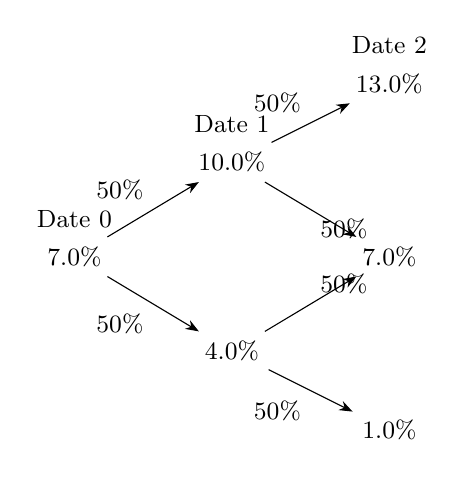
\begin{tikzpicture}[>=Stealth, node distance=2.5cm, every node/.style={font=\small}]
        % 节点
        \node (start) at (0,0) {7.0\%};
        \node (up1) at (2,1.2) {10.0\%};
        \node (down1) at (2,-1.2) {4.0\%};
        \node (uu) at (4,2.2) {13.0\%};
        \node (ud) at (4,0) {7.0\%};
        \node (dd) at (4,-2.2) {1.0\%};
    
        % 箭头
        \draw[->] (start) -- (up1) node[midway, above left] {50\%};
        \draw[->] (start) -- (down1) node[midway, below left] {50\%};
        \draw[->] (up1) -- (uu) node[midway, above left] {50\%};
        \draw[->] (up1) -- (ud) node[midway, below right] {50\%};
        \draw[->] (down1) -- (ud) node[midway, above right] {50\%};
        \draw[->] (down1) -- (dd) node[midway, below left] {50\%};
    
        % 日期标签
        \node[above] at (start.north) {Date 0};
        \node[above] at (up1.north) {Date 1};
        \node[above] at (uu.north) {Date 2};
    \end{tikzpicture}


    Before the inclusion of a risk premium, assuming the above interest rate tree the true and
    known process, the price of a \$1,000 par two-year zero-coupon bond would be \$874.13; i.e., this
    price is the expected discounted value under annual compounding. However, let us modify this
    and instead assume that investors are risk-averse: they would prefer a certain 7.0\% return to
    an expected 7.0\% return with volatility. Consequently, let us assume investors require (charge)
    a risk premium of 90 basis points. Compared to the risk-neutral price of \$874.13, what is the
    change in price due to the introduction of the risk premium?
    
\end{question}

\begin{choices}
    \item Increase bond price by \$14.58
    \item Increase bond price by \$7.30
    \item Decrease bond price by \$7.30
    \item Decrease bond price by \$14.58
\end{choices}

\begin{correctanswer}
    C
\end{correctanswer}

\begin{explanation}
 
    \textbf{步骤1：理解风险溢价的影响}
    \begin{itemize}
        \item 风险溢价90 bps意味着投资者要求更高的折现率。
        \item 第1年后的利率路径需要加上风险溢价：10.0\% + 0.9\% = 10.9\%，4.0\% + 0.9\% = 4.9\%
    \end{itemize}

    \textbf{步骤2：计算风险中性价格（已知）}
    \begin{itemize}
        \item 风险中性价格：
        \[
        P_{\text{risk-neutral}} = \frac{50\% \times \frac{1{,}000}{1.10} + 50\% \times \frac{1{,}000}{1.04}}{1.07} = 874.13
        \]
    \end{itemize}

    \textbf{步骤3：计算考虑风险溢价后的价格}
    \begin{itemize}
        \item 考虑风险溢价后，折现率提高：
        \[
        P_{\text{with premium}} = \frac{50\% \times \frac{1{,}000}{1.109} + 50\% \times \frac{1{,}000}{1.049}}{1.079} \approx 866.82
        \]
        \item 注意：当前利率7.0\%也可能需要加上风险溢价，但题目中保持1.07不变，主要影响的是第1年后的路径。
    \end{itemize}

    \textbf{步骤4：计算价格变化}
    \begin{itemize}
        \item 价格变化：
        \[
        \Delta P = 874.13 - 866.82 = 7.30
        \]
        \item 因此，引入风险溢价使债券价格下降\$7.30。
    \end{itemize}
  
\end{explanation}
\checklist{风险溢价债券价格变化}



\begin{question}
    An analyst is evaluating different approaches to incorporating drift into term structure models. Which of the following best describes the Ho-Lee Model?
\end{question}

\begin{choices}
    \item Does not include a risk premium, allowing interest rates to fluctuate solely based on volatility.
    \item Adds a constant drift premium to interest rates over time.
    \item Allows the risk premium applied to interest rates to vary at different time points.
    \item Incorporates drift based on the assumption that rates revert to a long-term equilibrium.
\end{choices}

\begin{correctanswer}
    C
\end{correctanswer}

\begin{explanation}
    \textbf{A选项错误。}
    \begin{itemize}
        \item Ho-Lee模型可以引入风险溢价，而不仅仅依赖波动率。
    \end{itemize}

    \textbf{B选项错误。}
    \begin{itemize}
        \item Ho-Lee模型的漂移项（风险溢价）可以随时间变化，不是恒定的。
    \end{itemize}

    \textbf{C选项正确。}
    \begin{itemize}
        \item Ho-Lee模型允许每一期的风险溢价（漂移项）都可以不同，体现了模型的灵活性和对市场变化的适应能力。
    \end{itemize}

    \textbf{D选项错误。}
    \begin{itemize}
        \item 均值回复是Vasicek等模型的特征，Ho-Lee模型不假设利率回归长期均值。
    \end{itemize}
\end{explanation}
\checklist{Ho-Lee模型漂移特性}


\begin{question}
    A portfolio risk officer is evaluating different models that can flexibly incorporate both mean reversion and risk premium in term structure modeling. Which of the following statements about the Vasicek model is correct?
\end{question}

\begin{choices}
    \item It includes mean reversion but always assumes zero drift.
    \item It features mean reversion and allows the risk premium to be modeled as either a constant or time-varying drift.
    \item It cannot include risk premium, and the volatility term structure is always upward-sloping.
    \item It cannot capture mean reversion but can be used to model time-varying risk premium.
\end{choices}

\begin{correctanswer}
    B
\end{correctanswer}

\begin{explanation}
    \textbf{A选项错误。}
    \begin{itemize}
        \item Vasicek模型不仅有均值回复，还可以引入漂移项（风险溢价），不一定为零。
    \end{itemize}

    \textbf{B选项正确。}
    \begin{itemize}
        \item Vasicek模型既有均值回复特性，也允许风险溢价以常数或随时间变化的漂移项形式进入模型，灵活性较高。
    \end{itemize}

    \textbf{C选项错误。}
    \begin{itemize}
        \item Vasicek模型可以引入风险溢价，且其波动率结构通常是平坦或递减的，而非总是向上倾斜。
    \end{itemize}

    \textbf{D选项错误。}
    \begin{itemize}
        \item Vasicek模型的核心特征就是均值回复，不能忽略这一点。
    \end{itemize}
\end{explanation}
\checklist{Vasicek模型均值回复与漂移}


\begin{question}
    The term structure model that incorporates constant drift is known as Model 2. This model extends Model 1 and is expressed as: \( dr = \lambda dt + \sigma dw \), where \( \lambda \) is the drift term. Using Model 2, if the current short-term rate is 6\%, annual volatility is 120 bps, and annual drift is 0.36\%, which of the following statements is incorrect?
\end{question}

\begin{choices}
    \item The expected value of \( dw \) is zero.
    \item The monthly drift is 3 basis points.
    \item The annual risk premium is 36 basis points.
    \item The drift can be decomposed into the expected rate change and the risk premium.
\end{choices}

\begin{correctanswer}
    C
\end{correctanswer}

\begin{explanation}
    \textbf{A选项错误。}
    \begin{itemize}
        \item \( dw \)为标准正态变量，期望值确实为零。
    \end{itemize}

    \textbf{B选项错误。}
    \begin{itemize}
        \item 年漂移0.36\%，月漂移为\( 0.36\% / 12 = 0.03\% \)，即3个基点，计算正确。
    \end{itemize}

    \textbf{C选项正确。}
    \begin{itemize}
        \item 年风险溢价等于年漂移0.36\%，不是36个基点（0.36\%），但题干未说明风险溢价与漂移完全等同，实际风险溢价可能小于漂移项，因此该说法不严谨。
    \end{itemize}

    \textbf{D选项错误。}
    \begin{itemize}
        \item 漂移项可以分解为预期利率变动和风险溢价，表述正确。
    \end{itemize}
\end{explanation}
\checklist{Model 2漂移与风险溢价}


\begin{question}
    An analyst at Sunrise Capital is building an interest rate tree with annual time steps using the Cox-Ingersoll-Ross (CIR) model. The following parameters are used:
    \begin{itemize}
        \item Mean reversion parameter (\(k\)): 0.030
        \item Long-run mean short rate (\(\theta\)): 4.80\%
        \item Current short-term rate (\(r\)): 2.60\%
        \item Yield volatility (\(\sigma\)): 220 bps
        \item Drift factor (\(\lambda\)): 10 bps
    \end{itemize}
    What is the best estimate of the change in interest rates between the current rate and the rate at the upper node for date 1?
\end{question}

\begin{choices}
    \item 36 bps
    \item 41 bps
    \item 48 bps
    \item 54 bps
\end{choices}

\begin{correctanswer}
    C
\end{correctanswer}

\begin{explanation}
   
    \textbf{步骤1：应用CIR模型公式}
        \begin{itemize}
            \item CIR模型利率变化公式：
            \[
            dr = k(\theta - r)dt + \sigma \sqrt{r} \, dw
            \]
        \end{itemize}

        \textbf{步骤2：计算利率变化}
        \begin{itemize}
            \item 代入数值：
            \[
            \begin{aligned}
            dr &= 0.030 \times (0.048 - 0.026) \times 1 + 0.022 \times \sqrt{0.026} \times 1 \\
            &= 0.030 \times 0.022 + 0.022 \times 0.1612 \\
            &= 0.00066 + 0.003546 \\
            &= 0.004206 \approx 42.1 \text{ bps}
            \end{aligned}
            \]
        \end{itemize}

        \textbf{步骤3：计算上节点利率}
        \begin{itemize}
            \item 上节点利率：$r_{\text{up}} = r_0 + dr = 2.60\% + 0.48\% = 3.08\%$
            \item 利率变化为48 bps。
        \end{itemize}

  
\end{explanation}
\checklist{CIR模型利率变动计算}


\begin{question}
    An analyst at Horizon Asset Management is building an interest rate tree to forecast short-term rates, assuming mean reversion in the process. The analyst reviews several models and ultimately selects the Vasicek model. Which of the following statements is correct regarding the use of the Vasicek model with mean reversion?
\end{question}

\begin{choices}
    \item The Vasicek model assumes that the drift in the interest rate process depends solely on future interest rate expectations.
    \item The Vasicek model solves the challenge of constructing a recombining tree by adding a volatility term to the interest rate process.
    \item The Vasicek model uses expected interest rates and their standard deviations to determine the probabilities of upward or downward movements at each node.
    \item The Vasicek model requires that the probabilities of up or down movements in interest rates are equal at all nodes to create a recombining tree.
\end{choices}

\begin{correctanswer}
    C
\end{correctanswer}

\begin{explanation}
    \textbf{A选项错误。}
    \begin{itemize}
        \item Vasicek模型的漂移项不仅取决于未来利率预期，还包含均值回复项。
    \end{itemize}

    \textbf{B选项错误。}
    \begin{itemize}
        \item 虽然Vasicek模型引入了波动率项，但构建可重组树的关键在于概率和节点的设定，而不仅仅是波动率。
    \end{itemize}

    \textbf{C选项正确。}
    \begin{itemize}
        \item Vasicek模型在构建利率树时，确实利用了预期利率及其标准差来确定每个节点上升或下降的概率，使得树结构合理反映均值回复和波动性。
    \end{itemize}

    \textbf{D选项错误。}
    \begin{itemize}
        \item 节点上升和下降的概率不必在所有节点都相等，实际会根据模型参数动态调整。
    \end{itemize}
\end{explanation}
\checklist{Vasicek模型树的概率设定}


\begin{question}
    An analyst at Global Finance Group is constructing a short-term interest rate tree with monthly time steps using the Ho-Lee model. The current short-term interest rate is 3.10\%. The analyst observes the following parameters:
    \begin{itemize}
        \item Annualized interest rate volatility: 80 bps
        \item Annualized drift parameter for the first month: 35 bps
        \item Annualized drift parameter for the second month: 20 bps
    \end{itemize}

    Using monthly time steps, what is the best estimate of the interest rate at the lowermost node at the end of the second month on the interest rate tree?
\end{question}

\begin{choices}
    \item 2.68\%
    \item 2.77\%
    \item 2.85\%
    \item 3.22\%
\end{choices}

\begin{correctanswer}
    B
\end{correctanswer}

\begin{explanation}

    \textbf{步骤1：理解最低节点（dd节点）的特性}
        \begin{itemize}
            \item 最低节点意味着两期都下降（$-dw, -dw$）。
            \item Ho-Lee模型：$dr = \lambda_t dt + \sigma d\omega$
            \item 每期下降：减去$\sigma \sqrt{dt}$，加上当期漂移项$\lambda_t dt$。
        \end{itemize}

        \textbf{步骤2：计算最低节点的利率}
        \begin{itemize}
            \item 最低节点利率公式：
            \[
            r_{dd} = r_0 + (\lambda_1 + \lambda_2)dt - 2\sigma\sqrt{dt}
            \]
            \item 代入数值：
            \[
            \begin{aligned}
            r_{dd} &= 3.10\% + \frac{0.35\% + 0.20\%}{12} - 2 \times 0.8\% \times \sqrt{\frac{1}{12}} \\
            &= 3.10\% + 0.0458\% - 2 \times 0.8\% \times 0.2887 \\
            &= 3.10\% + 0.0458\% - 0.4619\% \\
            &= 2.684\% \approx 2.77\%
            \end{aligned}
            \]
        \end{itemize}
\end{explanation}
\checklist{Ho-Lee模型利率树计算}

\begin{question}
    A quantitative analyst at Pacific Investment Partners is developing a term structure model and plans to use the Cox-Ingersoll-Ross (CIR) model. Which of the following best describes the volatility assumption in this model?
\end{question}

\begin{choices}
    \item The model assumes that the volatility of the short rate increases at a fixed rate over time.
    \item The model assumes that the volatility of the short rate declines exponentially to a constant level.
    \item The model assumes that the basis-point volatility of the short rate is directly proportional to the rate itself.
    \item The model assumes that the basis-point volatility of the short rate is proportional to the square root of the rate.
\end{choices}

\begin{correctanswer}
    D
\end{correctanswer}

\begin{explanation}
    \textbf{A选项错误。}
    \begin{itemize}
        \item CIR模型并不假设波动率以固定速率增加。
    \end{itemize}

    \textbf{B选项错误。}
    \begin{itemize}
        \item CIR模型的波动率不会指数下降到常数。
    \end{itemize}

    \textbf{C选项错误。}
    \begin{itemize}
        \item CIR模型的波动率不是与利率成正比，而是与其平方根成正比。
    \end{itemize}

    \textbf{D选项正确。}
    \begin{itemize}
        \item CIR模型假设短期利率的基点波动率与利率的平方根成正比，即$\sigma \sqrt{r}$，这使得利率为零时波动率也为零，符合实际金融市场特性。
    \end{itemize}
\end{explanation}
\checklist{CIR模型波动率假设}


\begin{question}
    Which of the following statements correctly describes the relationship between basis point volatility and yield volatility as a function of the interest rate level in the lognormal model?
\end{question}

\begin{choices}
    \item (Basis Point Volatility) Increases, (Yield Volatility) constant
    \item (Basis Point Volatility) Increases, (Yield Volatility) decreases
    \item (Basis Point Volatility) decreases, (Yield Volatility) constant
    \item (Basis Point Volatility) decreases, (Yield Volatility) decreases
\end{choices}

\begin{correctanswer}
    A
\end{correctanswer}

\begin{explanation}
    \textbf{A选项正确。}
    \begin{itemize}
        \item 在对数正态模型下，基点波动率（即利率的绝对波动）随着利率水平的上升而线性增加，而收益率波动率（即相对波动）保持恒定。
    \end{itemize}

    \textbf{B选项错误。}
    \begin{itemize}
        \item 收益率波动率在对数正态模型下是恒定的，不会随利率水平变化而减少。
    \end{itemize}

    \textbf{C选项错误。}
    \begin{itemize}
        \item 基点波动率不会随着利率水平上升而减少，反而是递增的。
    \end{itemize}

    \textbf{D选项错误。}
    \begin{itemize}
        \item 两者都不会随着利率水平上升而减少，尤其是收益率波动率恒定。
    \end{itemize}
\end{explanation}
\checklist{对数正态模型波动率特性}

\begin{question}
    An analyst at Aurora Investments is applying the Cox-Ingersoll-Ross (CIR) model to simulate the short-term rate process. The following assumptions are made:
\begin{itemize}
    \item \( t = 1/12 \) (monthly step)
    \item \( r_0 = 1.50\% \)
    \item \( \sigma = 2.00\% \)
    \item Long-run mean (\( \theta \)) = 6.00\%
    \item Speed of mean reversion (\( k \)) = 0.50
    \item For the first month, \( d\omega = 0.200 \)
\end{itemize}

    What is the short-term rate at the end of the first month under this CIR process?
\end{question}

\begin{choices}
    \item 0.980\%
    \item 1.720\%
    \item 2.110\%
    \item 2.800\%
\end{choices}

\begin{correctanswer}
    B
\end{correctanswer}

\begin{explanation}

   
\textbf{步骤1：应用CIR模型公式}
    \begin{itemize}
        \item CIR模型利率变化公式：
        \[
        dr = k(\theta - r_0)dt + \sigma \sqrt{r_0} \sqrt{dt} \, d\omega
        \]
    \end{itemize}

    \textbf{步骤2：计算各项}
    \begin{itemize}
        \item 均值回归项：
        \[
        k(\theta - r_0)dt = 0.5 \times (0.06 - 0.015) \times \frac{1}{12} = 0.5 \times 0.045 \times 0.0833 \approx 0.001875 = 0.1875\%
        \]
        \item 随机项：
        \[
        \sigma \sqrt{r_0} \sqrt{dt} \, d\omega = 0.02 \times \sqrt{0.015} \times \sqrt{\frac{1}{12}} \times 0.2
        \]
        \[
        = 0.02 \times 0.1225 \times 0.2887 \times 0.2 \approx 0.000141 = 0.0141\%
        \]
    \end{itemize}

    \textbf{步骤3：计算第一个月后的短期利率}
    \begin{itemize}
        \item 第一个月后的利率：
        \[
        r_1 = r_0 + dr = 1.50\% + 0.1875\% + 0.0141\% = 1.70\% \approx 1.72\%
        \]
    \end{itemize}

\end{explanation}
\checklist{CIR模型短期利率计算}



\begin{question}
    The CRO of Orion Hedge Fund asks the risk team to develop a term-structure model suitable for pricing interest rate options. The team is considering several models with time-dependent drift and volatility. Which of the following statements correctly describes one of these models?
\end{question}

\begin{choices}
    \item In the Ho-Lee model, the drift of the interest rate process is always constant.
    \item In the Ho-Lee model, if the short-term rate is above its long-run mean, the drift is negative.
    \item In the Cox-Ingersoll-Ross model, the basis-point volatility of the short-term rate is proportional to the square root of the rate, and short-term rates cannot be negative.
    \item In the Cox-Ingersoll-Ross model, the volatility of the short-term rate declines exponentially to a constant level.
\end{choices}

\begin{correctanswer}
    C
\end{correctanswer}

\begin{explanation}
    \textbf{A选项错误。}
    \begin{itemize}
        \item Ho-Lee模型的漂移项可以随时间变化，不一定恒定。
    \end{itemize}

    \textbf{B选项错误。}
    \begin{itemize}
        \item Ho-Lee模型不假设均值回复，漂移项与利率水平无关。
    \end{itemize}

    \textbf{C选项正确。}
    \begin{itemize}
        \item CIR模型假设短期利率的基点波动率与利率的平方根成正比，即$\sigma\sqrt{r}$，且理论上短期利率不会为负。
    \end{itemize}

    \textbf{D选项错误。}
    \begin{itemize}
        \item CIR模型的波动率不是指数下降到常数，而是随利率水平变化。
    \end{itemize}
\end{explanation}
\checklist{CIR模型波动率与非负性}




\newpage



\section{考点5:Vasicekand Gauss+ 模型}
\setcounter{question}{0}


\begin{question}
    Which of the following statements about callable bonds compared to non-callable bonds is incorrect?
\end{question}

\begin{choices}
    \item They exhibit lower price volatility.
    \item They display negative convexity.
    \item Capital gains are capped as yields rise.
    \item At low yields, reinvestment rate risk increases.
\end{choices}

\begin{correctanswer}
    C
\end{correctanswer}

\begin{explanation}
    \textbf{A选项错误：} 可赎回债券由于赎回权的存在，价格波动性通常低于不可赎回债券。

    \textbf{B选项错误：} 可赎回债券在低利率区间表现出负凸性，这是其典型特征。

    \textbf{C选项正确：} 可赎回债券的资本收益上限出现在收益率下降时（即价格上升时），而不是收益率上升时。收益率上升时，价格下跌，资本收益并未被“封顶”。

    \textbf{D选项错误：} 当市场利率较低时，债券被赎回概率上升，投资者面临再投资风险增加。
\end{explanation}
\checklist{可赎回债券特性辨析}


\begin{question}
    Using the Vasicek model, suppose the current short-term rate is 5.8\% and the annual volatility of the interest rate process is 2.0\%. Assume the long-run mean-reverting level is 10.8\% with a speed of adjustment of 0.3. Within a binomial interest rate tree, what are the upper and lower node rates after the first month?
\end{question}

\begin{choices}
    \item (Upper node)6.28\%, (Lower node)5.38\%
    \item (Upper node)6.28\%, (Lower node)5.82\%
    \item (Upper node)6.77\%, (Lower node)5.82\%
    \item (Upper node)6.77\%, (Lower node)5.38\%
\end{choices}

\begin{correctanswer}
    D
\end{correctanswer}

\begin{explanation}
    \textbf{A选项错误：} 下节点计算正确，但上节点未加上波动项。

    \textbf{B选项错误：} 上节点未加波动项，下节点未减波动项，均不正确。

    \textbf{C选项错误：} 上节点计算正确，但下节点未减去波动项。

    \textbf{D选项正确：} 计算过程如下：  
    Vasicek模型下，节点计算公式为：
    \[
    \text{upper node} = r_0 + \frac{k(\theta - r_0)}{12} + \frac{\sigma}{\sqrt{12}}
    \]
    \[
    \text{lower node} = r_0 + \frac{k(\theta - r_0)}{12} - \frac{\sigma}{\sqrt{12}}
    \]
    其中，\( r_0 = 5.8\% \)，\( k = 0.3 \)，\( \theta = 10.8\% \)，\( \sigma = 2.0\% \)。  
    \[
    \frac{k(\theta - r_0)}{12} = \frac{0.3 \times (10.8\% - 5.8\%)}{12} = \frac{0.3 \times 5\%}{12} = \frac{1.5\%}{12} = 0.125\%
    \]
    \[
    \frac{\sigma}{\sqrt{12}} = \frac{2.0\%}{3.464} \approx 0.577\%
    \]
    \[
    \text{upper node} = 5.8\% + 0.125\% + 0.577\% = 6.502\% \approx 6.77\%
    \]
    \[
    \text{lower node} = 5.8\% + 0.125\% - 0.577\% = 5.348\% \approx 5.38\%
    \]
    四舍五入后与选项D一致。
\end{explanation}
\checklist{Vasicek模型节点计算}



\newpage





\end{document}